\documentclass[12pt]{article}
\usepackage[paper=a4paper,left=30mm,right=30mm,top=35mm,bottom =35mm]{geometry}
\usepackage[utf8]{inputenc}
\usepackage[T1]{fontenc}
\usepackage{stmaryrd}
\usepackage{setspace}
\usepackage{mathrsfs}
\usepackage[ngerman]{babel}
\usepackage{amssymb}
\usepackage{amsmath}
\usepackage{fancyhdr}
\usepackage[dvips,unicode,colorlinks,linkcolor=black]{hyperref} 
\usepackage{graphicx}
\usepackage{float}

\pagestyle{fancy}
\lfoot{}
\rfoot{Paul Kremser, Tobias Grussenmeyer}
\cfoot{\thepage}
\fancyhead[L]{FPI Versuch: Rastertunnelmikroskop}
\renewcommand{\headrulewidth}{0.6pt}
\renewcommand{\footrulewidth}{0.6pt}
\setlength{\headheight}{16pt}
\setlength{\parindent}{0pt}
% Für die Wahl der Schriftart
\newcommand{\changefont}[3]{
\fontfamily{#1} \fontseries{#2} \fontshape{#3} \selectfont}

\begin{document}
% keine Hurenkinder und Schusterjungen
\clubpenalty = 10000
\widowpenalty = 10000 
\displaywidowpenalty = 10000

\onehalfspacing
% Schriftart
\changefont{ptm}{m}{n} 

\begin{titlepage}
\author{Paul Kremser, Tobias Grussenmeyer}
\title{Versuch: Rastertunnelmikroskop}
\date{Versuchsdurchführung: 19. und 26. November 2009} 
\maketitle
\thispagestyle{empty}
\end{titlepage}


\tableofcontents
\thispagestyle{empty}
\newpage
\pagenumbering{arabic}
\section{Überblick}
Bei der Rastertunnelmikroskopie wird eine Sonde, eine elektrisch leitende Nadel, meistens Spitze genannt über die Probe geführt. Der wechselwirkende Prozess ist der des quantenmechanischen Tunneleffekts. Bei einer angelegten Spannung zwischen einer Spitze und einer Oberfläche führt dies zu einem statisch messbaren Tunnelstrom. Der Tunnelstrom hängt vom Abstand zwischen Spitze und Probe ab. Durch Steuerung der Spitzte mittels Piezokristall lassen sich somit Höhenunterschiede in atomarer Größenordnung messen.

\section{Aufgabestellung}

\section{Theoretische Grundlagen}
Das Rastertunnelmikroskop bezeichnet den experimentellen Aufbau, in dem die Spitze zeilenweise über eine Oberfläche gerastert wird und der Tunnelstrom die zentrale Messgröße ist. Die Ortskoordinaten $(x,y)$ des Rasterfeldes sind ungeregelte Größen während der Tunnelstrom $I$ abhängig ist von der $z$-Position und der angelegten Spannung $U$ und meistens über eine Regelschleife miteinander verbunden ist. Die Abhängigkeit voneinander bildet dabei verschiedene physikalische Eigenschaften der Oberfläche ab. $I(U)$ bei konstantem $z$ wird Tunnelspektroskopie genannt und $I(z)$ bei $U = const$ gibt Zugang zur Austrittsarbeit. Das Auftragen der Ortsabhängigkeit verschiedener Größen wird i.A. abbilden genannt. Dabei wird eine sehr hohe Auflösung bis zur atomaren Skala erzielt, da der dem RTM zu Grunde liegende Tunneleffekt sensitiv auf Änderungen im Sub-Angstrom-Bereich ist. Die Ortsabhängigkeit des Tunnelstroms spiegelt die Konvolution der realen Topographie mit elektronischen Eigenschaften wieder. Eine dreidimensionale Auftragung suggeriert dabei einen pseudomäßigen Blick auf die Oberflächentopographie bildet aber exakter weise die Höhentopologie konstanter Elektronendichte ab.


\subsection{Fermienergie}
Als Fermienergie bezeichnet man das chemische Potenzial am absoluten Temperaturnullpunkt $T = 0K$
Das Pauli-Prinzip besagt, dass Fermionen sich mindestens in einer Quantenzahl unterscheiden müssen. Dies hat zur Folge, dass auch am absoluten Temperaturnullpunkt Fermionen in angeregten Energiezuständen sitzen müssen. Folglich hat die Fermi-Verteilung bei $T = 0 K$ also eine scharfe Kante bei einer Energie, deren Höhe von der Anzahl der Fermionen in dem betrachteten System abhängt und als Fermi-Kante, Fermi-Grenze oder Fermi-Energie $E_f$ bezeichnet wird. Ganz wichtig ist hierbei, dass die Fermi-Verteilung nur eine Wahrscheinlichkeit angibt, mit der ein Zustand besetzt wird. Ob der Zustand auch besetzt wird, hängt davon ab, ob ein entsprechender Zustand existiert. Bei einem Halbleiter existiert zur Fermi-Energie kein erlaubter Zustand, er kann nicht besetzt werden.

\subsection{Austrittsarbeit}
Die Austrittsarbeit ist die Arbeit, die mindestens aufgewandt werden muss, um ein Elektron aus einem ungeladenen Festkörper zu lösen. In der Regel wird die Austrittsarbeit in Elektronenvolt angegeben. Die Austrittsarbeit ist also die Energie beim Herausholen eines Elektrons aus dem Ferminiveau. Die Austrittsarbeit ist daher über das chemische Potential abhängig von der Art des Festkörpers, aus dem Elektronen ausgelöst werden. Sie ist relativ klein für Alkalimetalle, während sie für Metalle wie Aluminium, Zink oder Platin wesentlich höher ist.

\subsection{lokalisierte und delokalisierte Elektronen}
Von delokalisierten Elektronen spricht man immer dann, wenn sich die einzelnen Elektronen keinem bestimmten Atom zuordnen lassen. Die Elektronen haben also prinzipiell an jedem Gitteratom eine nichtverschwindende Aufenthaltswahrscheinlichkeit.
Lokalisierte Elektronen dagegen sind solche die an ein Atom gebunden oder einer bestimmten Bindung zugeordnet werden können.

\subsection{Tunneleffekt}
Der Tunneleffekt ist der quantenmechanische Effekt, der Teilchen die Überwindung endlicher Potentialbarrieren erlaubt, welche nach den Vorstellungen der klassischen Physik für diese Teilchen unüberwindbar wären.

Die quantenmechanische Betrachtungsweise geht von der Schrödingergleichung aus. Diese Wellenfunktion dringt in den verbotenen Bereich ein und klingt exponentiell ab. Durch den exponentiellen Abfall der Welle in dem verbotenen Bereich bleibt am Ende des verbotenen Bereiches noch ein Rest der ursprünglichen Welle übrig. Das Betrags-Quadrat der Wellenfunktion  wird als Wahrscheinlichkeitsdichte interpretiert, was bedeutet, dass es eine kleine Wahrscheinlichkeit für das Teilchen gibt, auf der anderen Seite der Barriere aufzutauchen.


\subsection{Struktur von Graphit und $MoS_2$}
\begin{figure}[H]
\centering
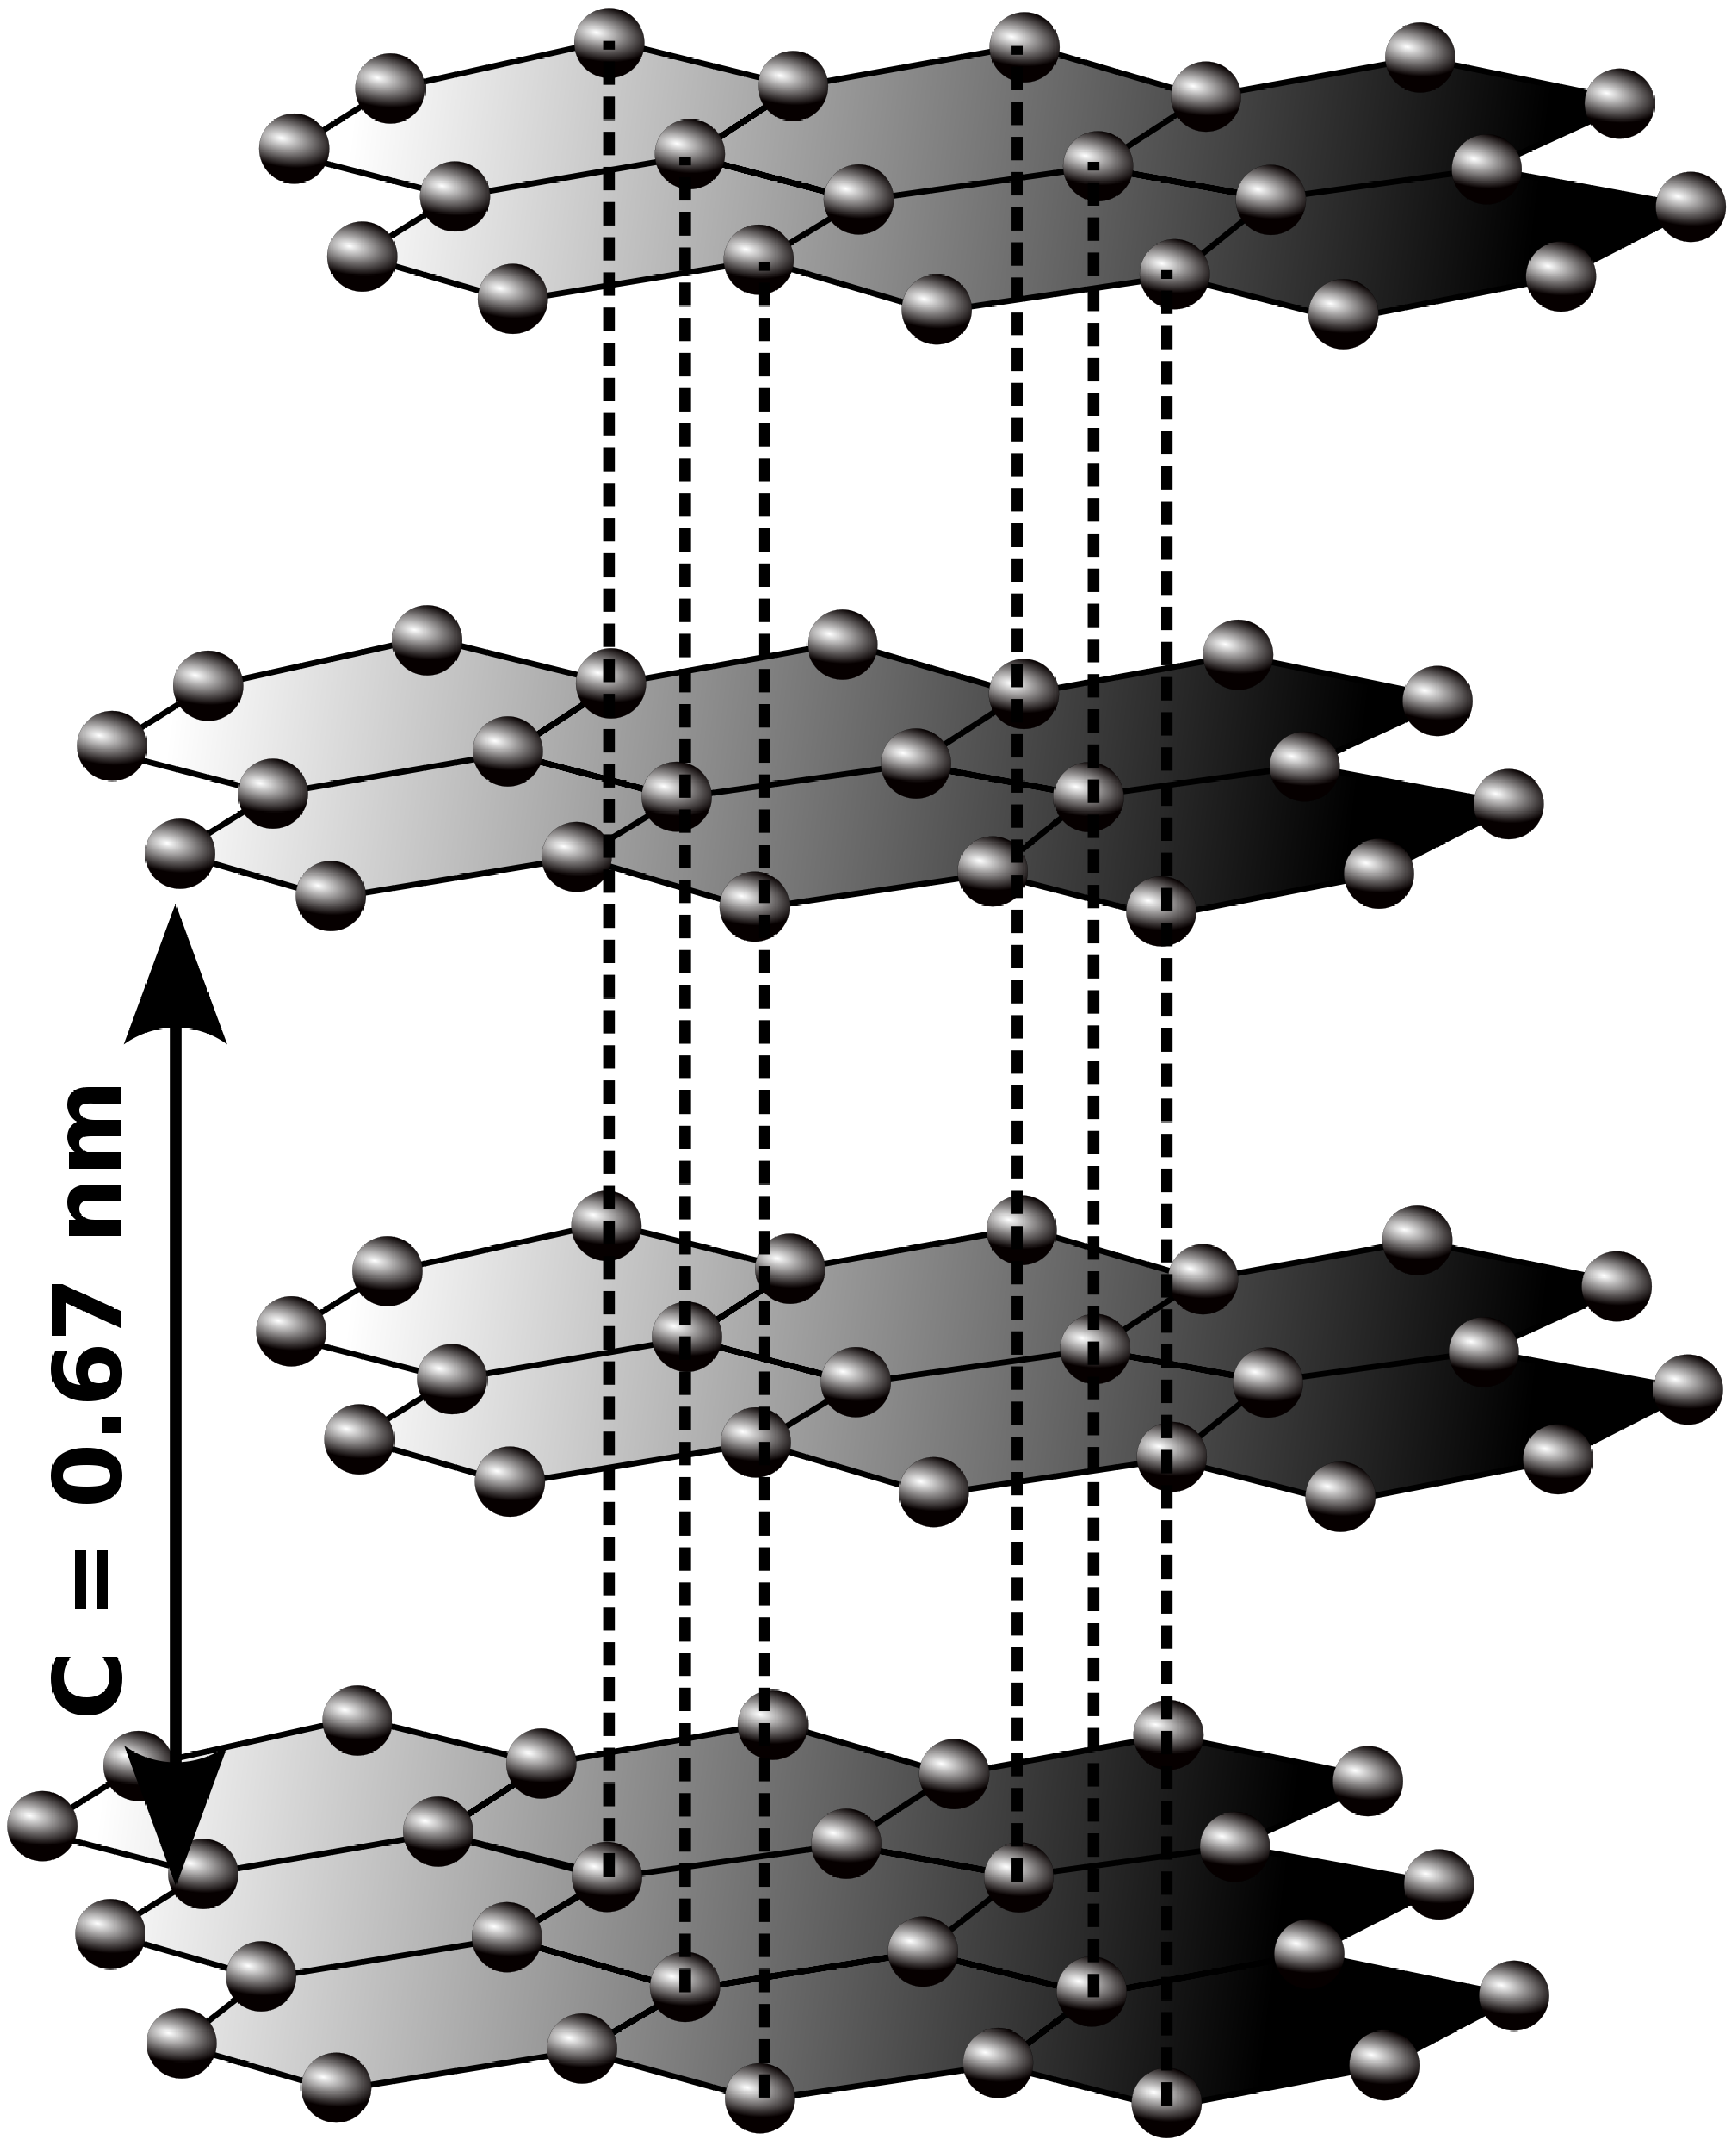
\includegraphics[width=0.6\linewidth]{pictures/graphitgitter.eps}
\caption{Graphitstruktur}
\end{figure}
Bei einer Rastertunnelaufnahme der Graphitoberfläche sind nur diejenigen Oberflächenatome, die kein unmittelbares Nachbaratom in der nächstunteren Schicht besitzen (mit Punktlinie verbundene Atompositionen im oberen Bild) zu sehen, da hier die elektronische Zustandsdichte höher ist. Ein unteres C-Atom als Nachbar würde durch schwache Bindung elektronische Dichte abziehen.
\begin{figure}[H]
\centering
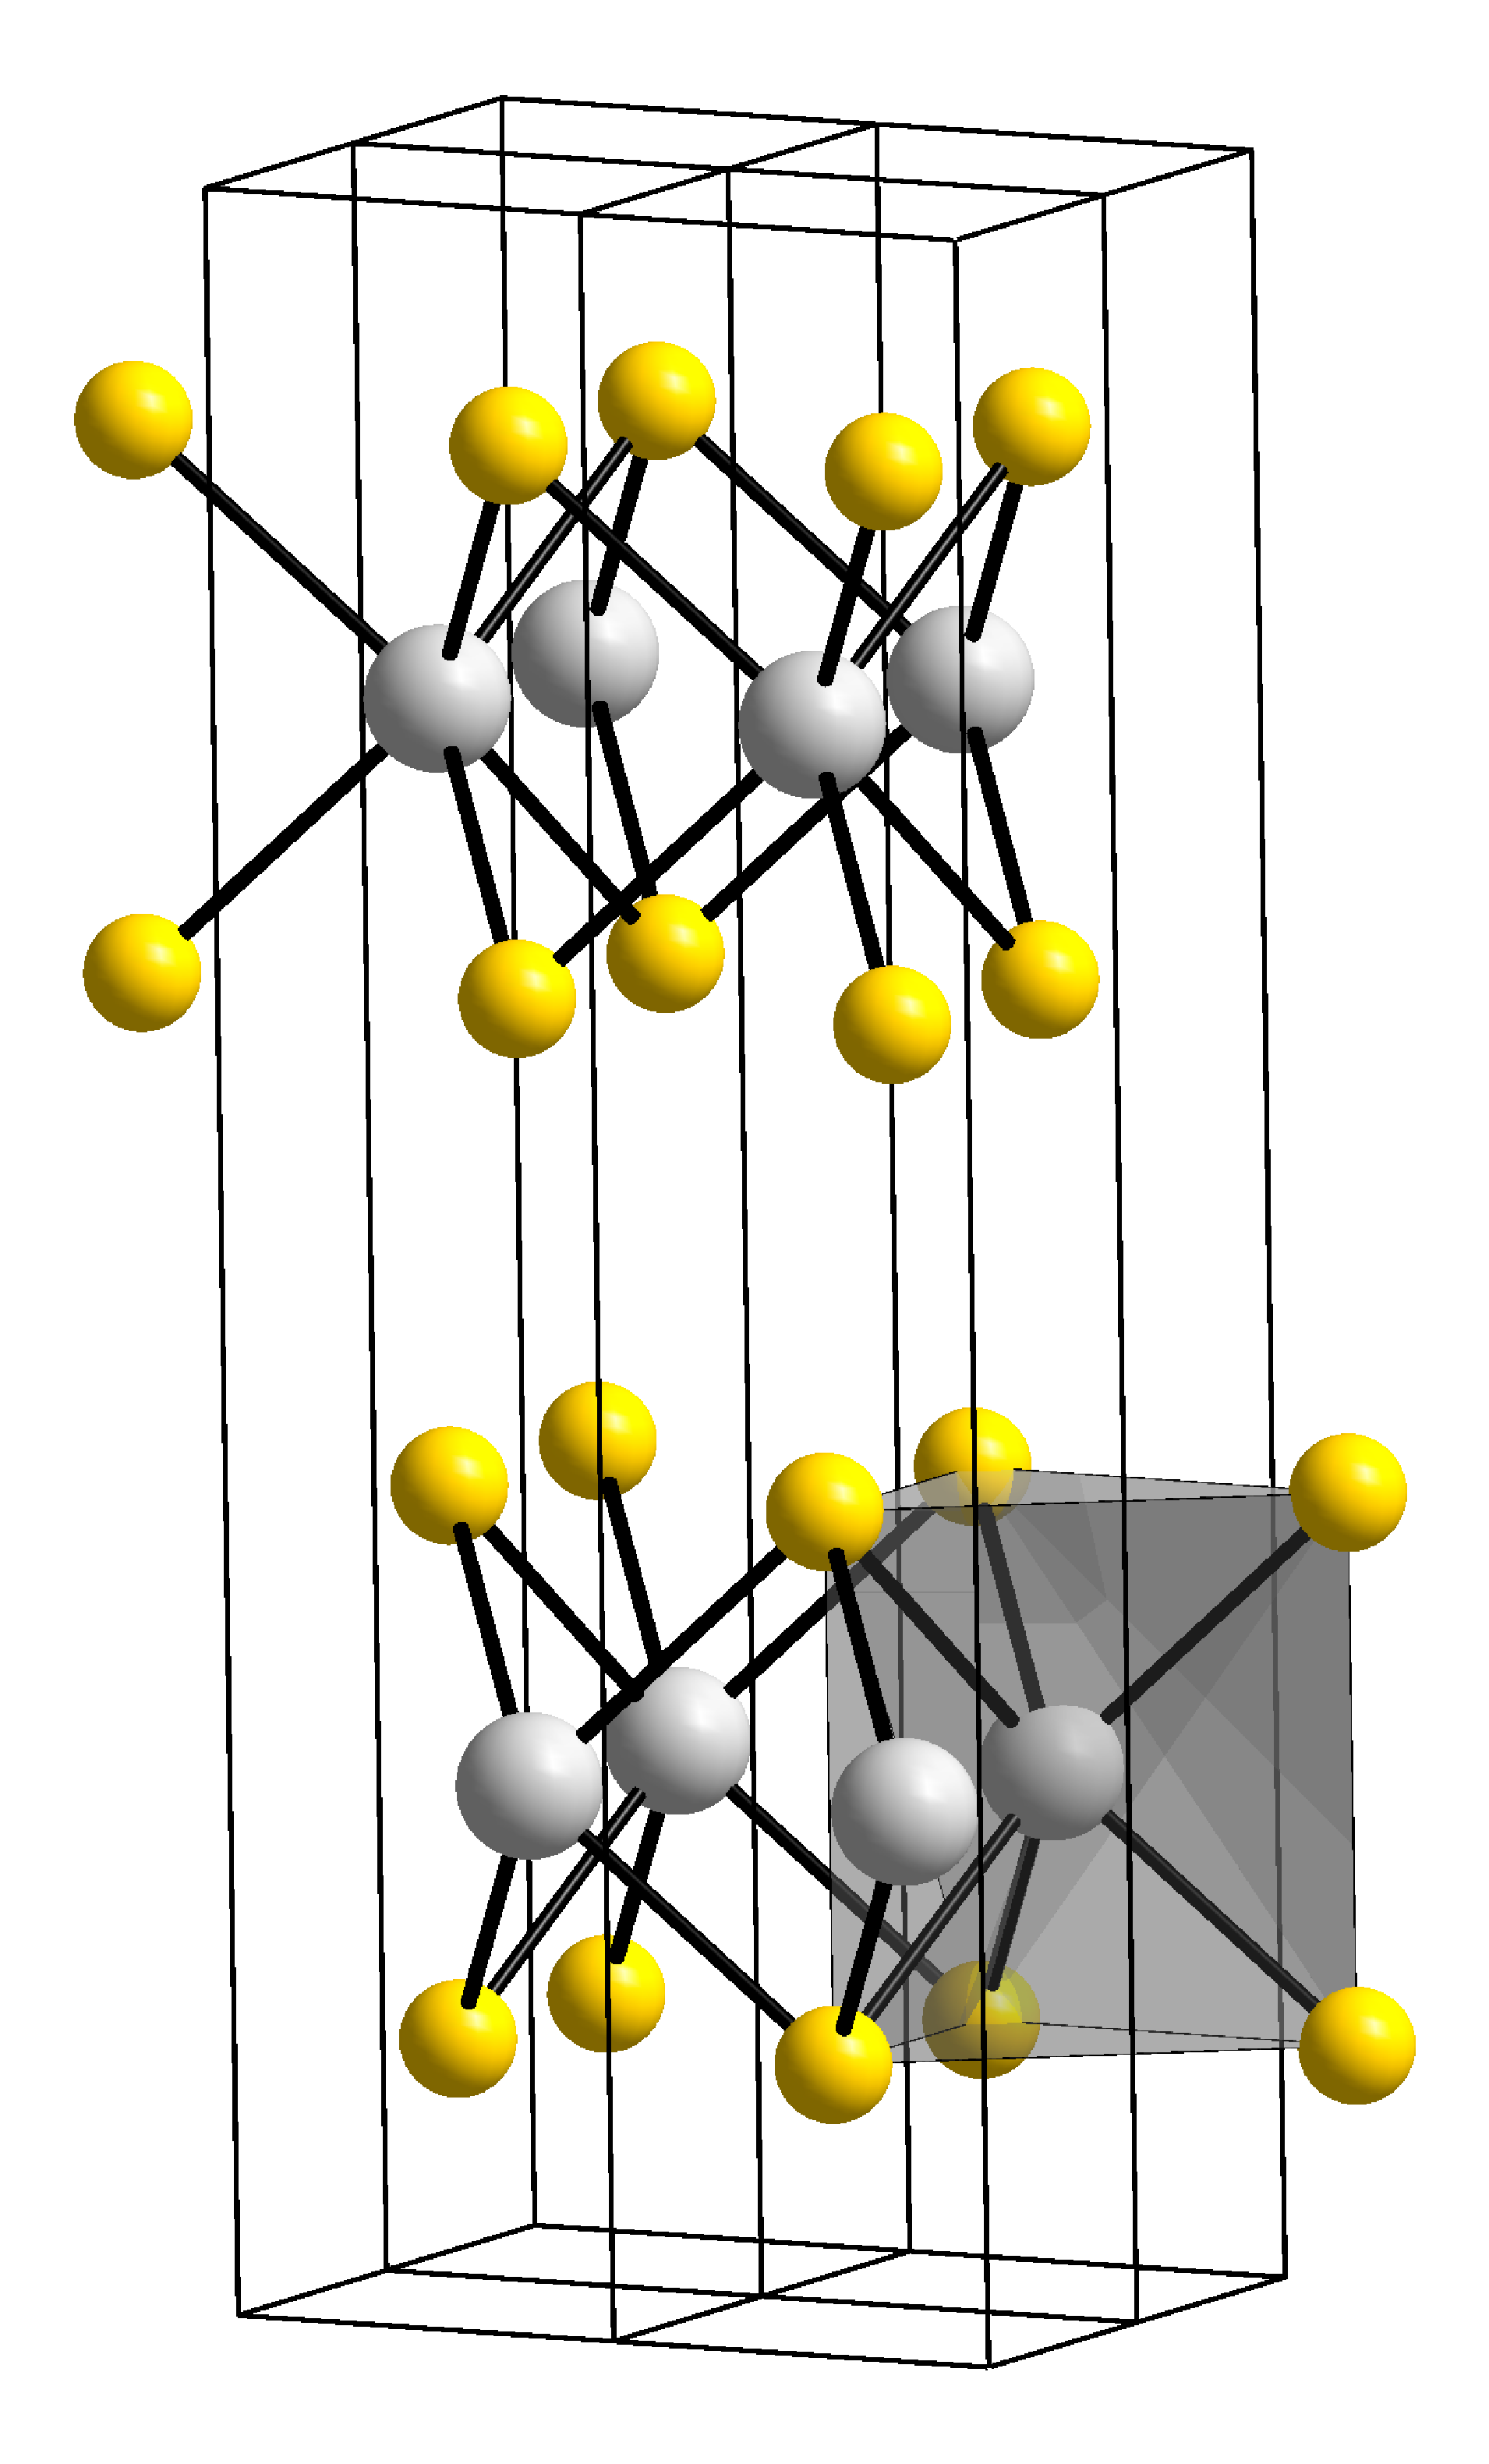
\includegraphics[width=0.6\linewidth]{pictures/mos2.eps}
\caption{Molybdändisulfid (gelb: $S^{2-}$, grau: $Mo^{4+}$)}
\end{figure}

\section{Versuchsaufbau}
\begin{figure}[H]
\centering
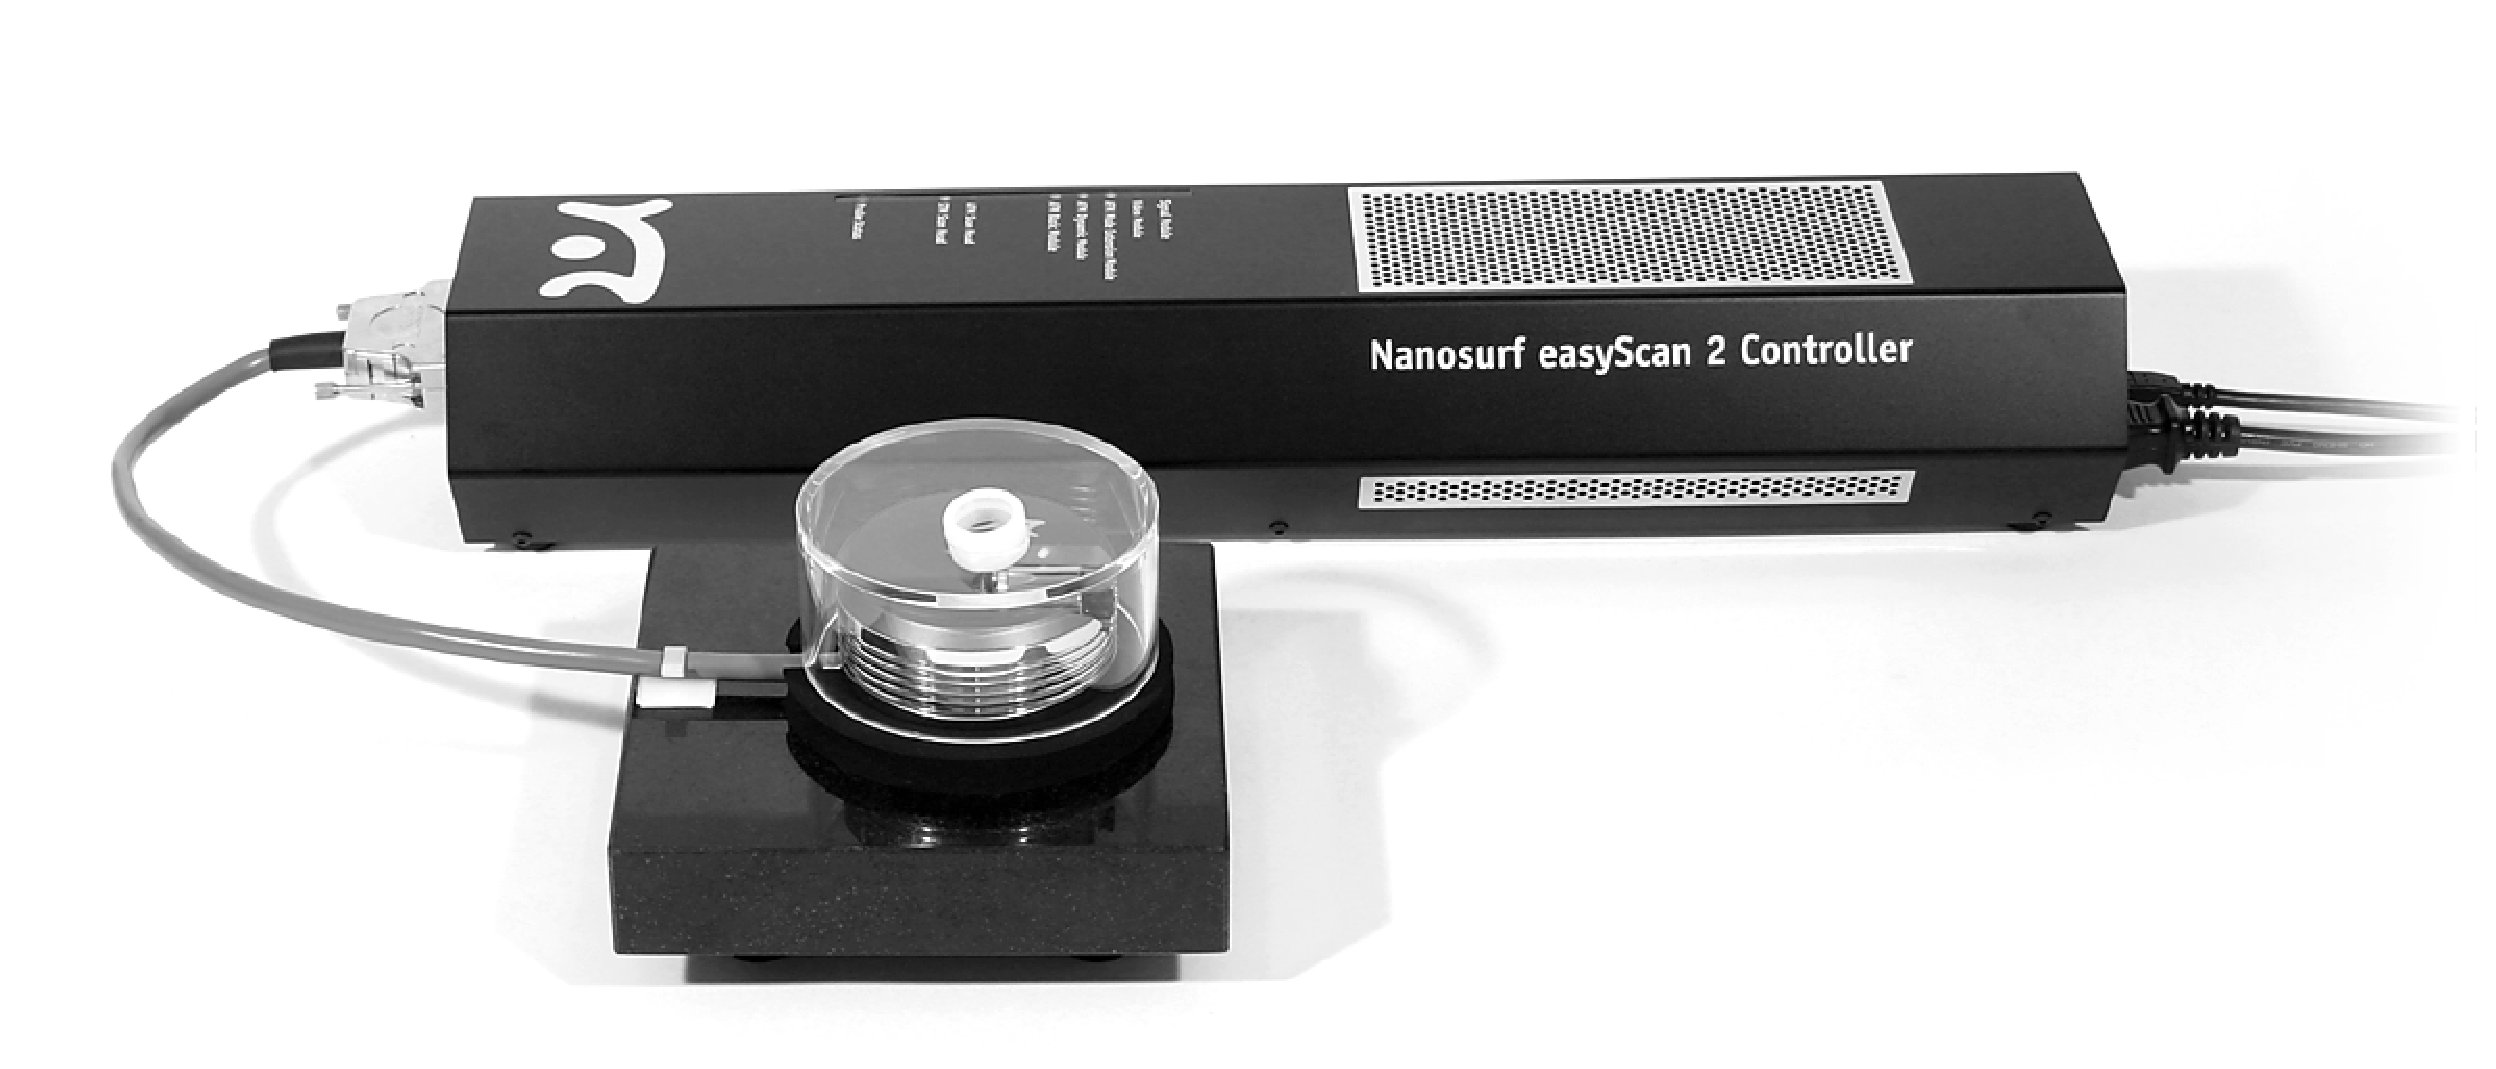
\includegraphics[width=0.9\linewidth]{pictures/aufbau.eps}
\caption{Das RTM mit Steuereinheit}
\end{figure}

\begin{figure}[H]
\centering
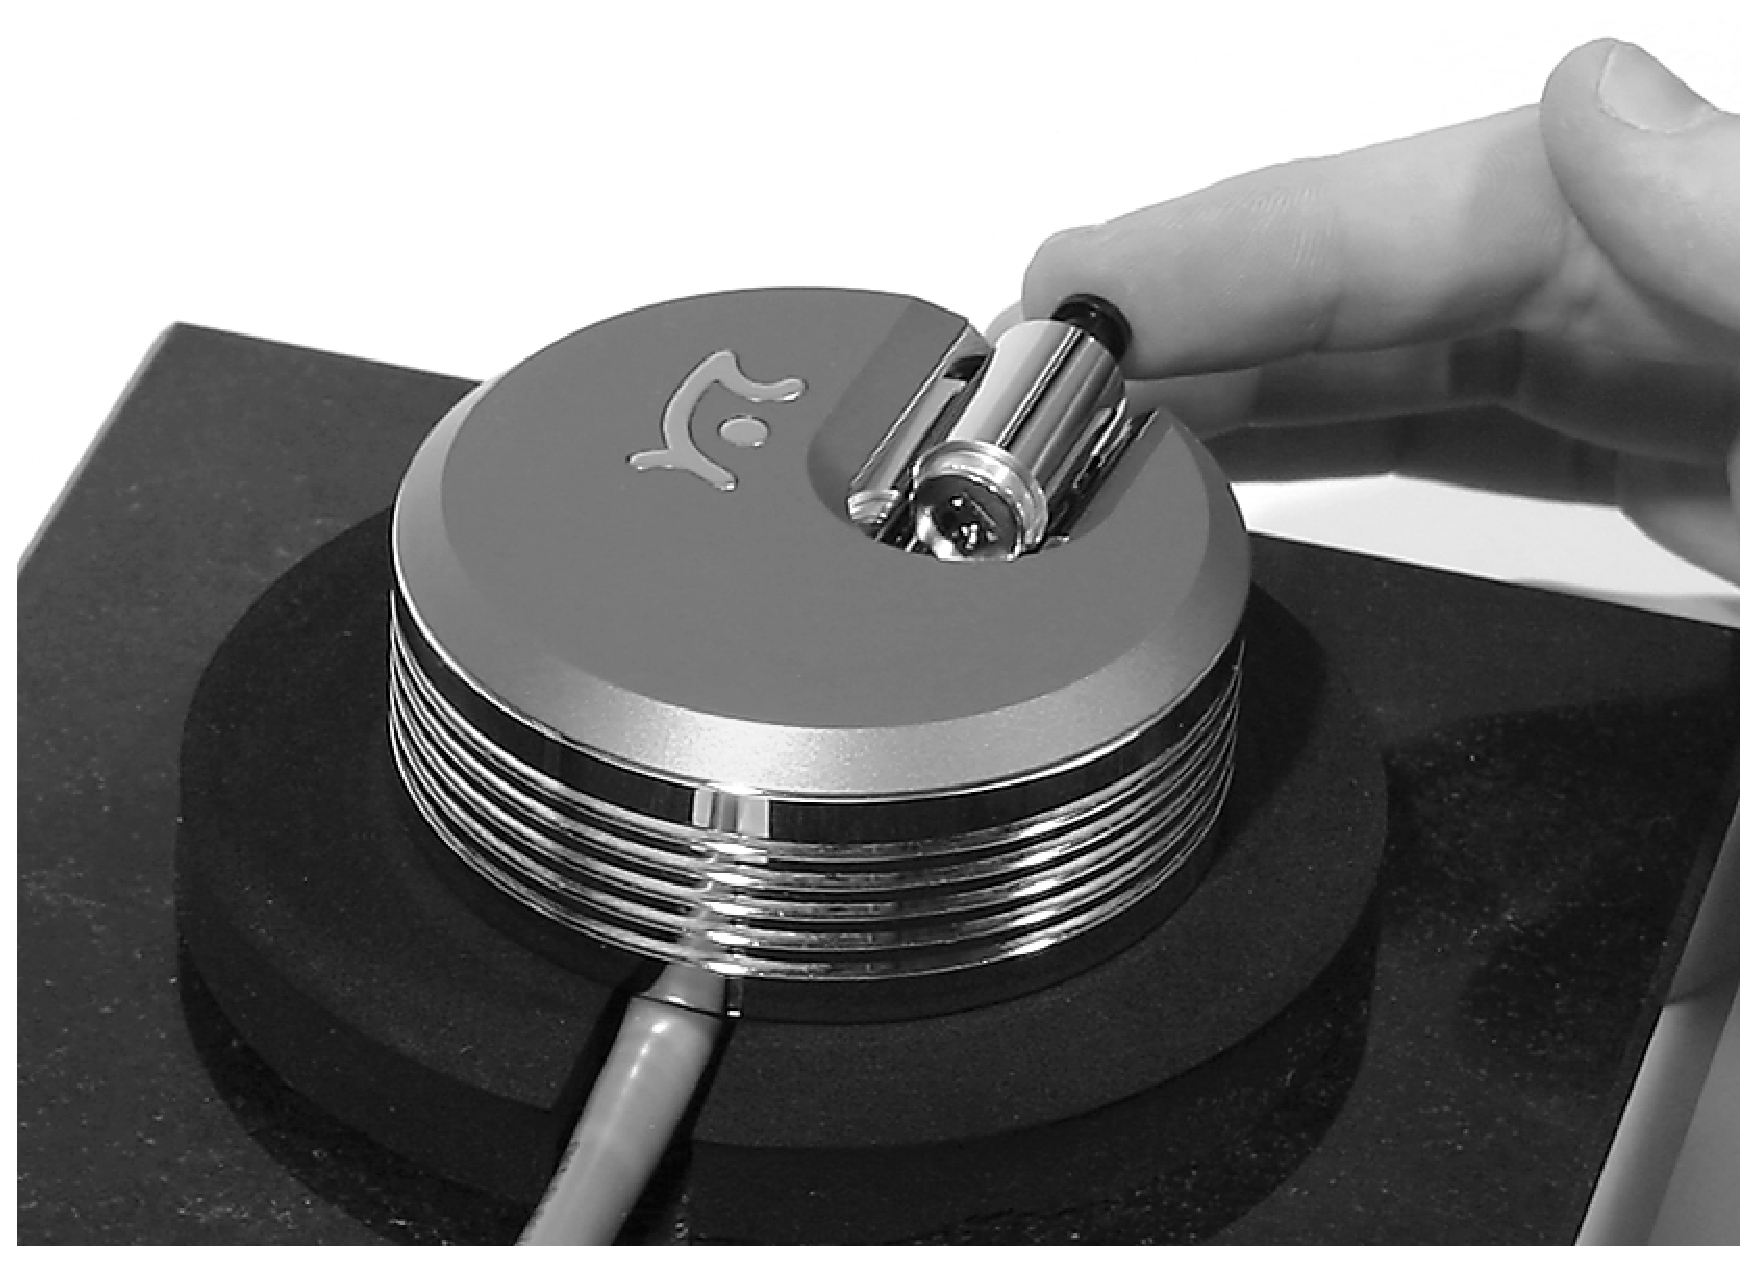
\includegraphics[width=0.9\linewidth]{pictures/rastertunnel.eps}
\caption{Das eigentliche RTM}
\end{figure}
\section{Durchführung}
Zu Beginn, wie auch noch mehrmals während des Versuchs muss eine Spitze hergestellt werden. Hierzu wird mit einem Seitenschneider ein Platin-Iridium-Draht angeschnitten und dann abgerissen. Die Spitze und Probe werden in das Mikroskop eingesetzt. Die Probe befindet sich auf einem Probenhalter welcher als Schlitten elektronisch gesteuert werden kann. Anfangs wird die Probe von Hand auf ca. $1mm$ Abstand zur Spitze gebracht und dann mittels der Elektronik weiter an die Probe angenähert.
Bei dem automatisierten Annäherungsprozess kam es oft vor das die Probe gegen die Spitze stieß und die Spitze ausgewechselt werden musste. \\

Unter Verwendung etlicher Spitzen haben wir schlussendlich Bilder der drei Proben aufgenommen
\section{Auswertung}
\subsection{Gold}
\begin{figure}[H]  
\begin{minipage}{0.4\linewidth}
\centering
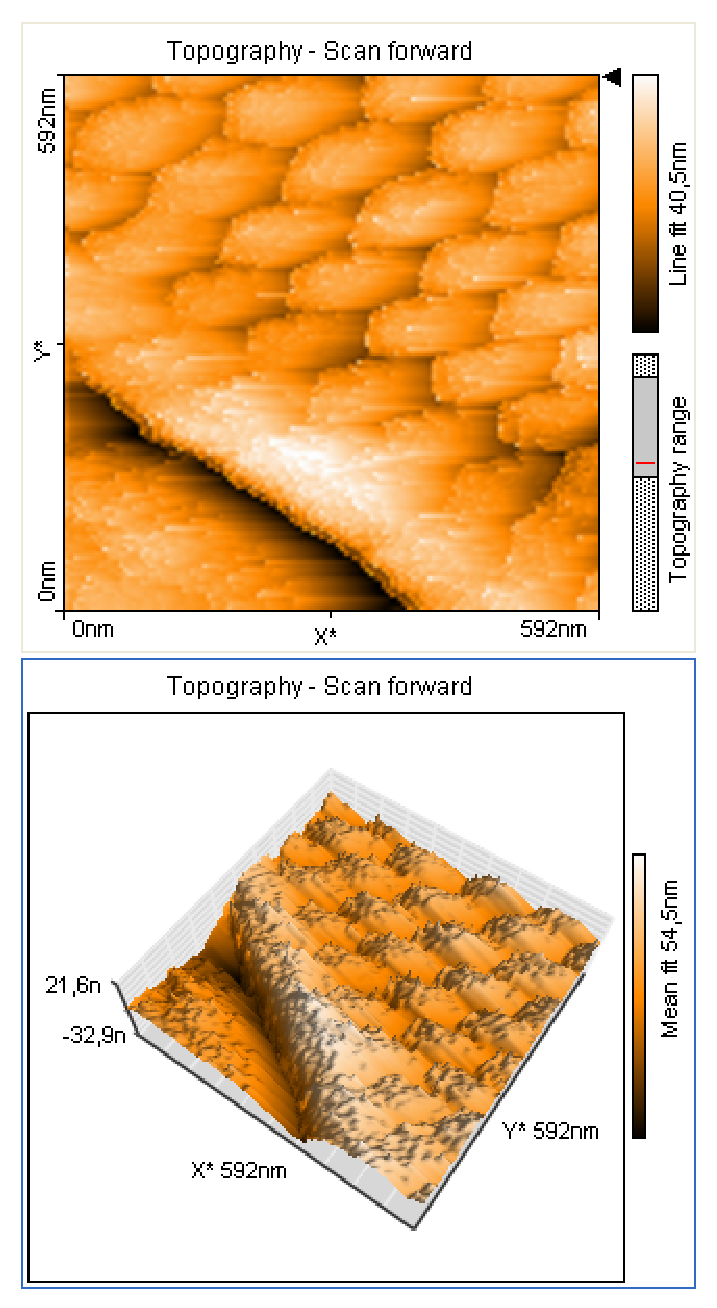
\includegraphics[width=0.9\linewidth]{../plot/data/goldgitter/goldgitter.eps}
\end{minipage}
\begin{minipage}{0.2\linewidth}
\centering
\end{minipage}
\begin{minipage}{0.4\linewidth}
\centering
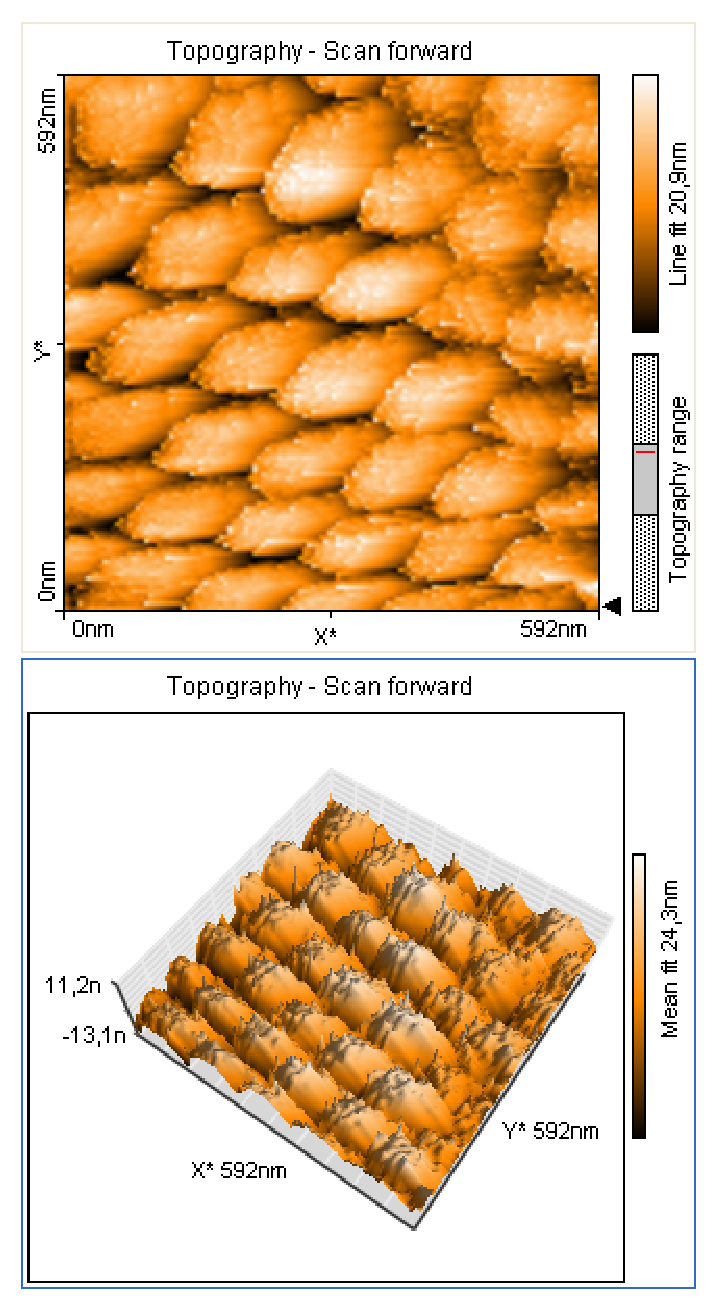
\includegraphics[width=0.9\linewidth]{../plot/data/goldgitter/goldgitter2.eps}
\end{minipage}
\end{figure}

\begin{figure}[H]  
\begin{minipage}{0.4\linewidth}
\centering
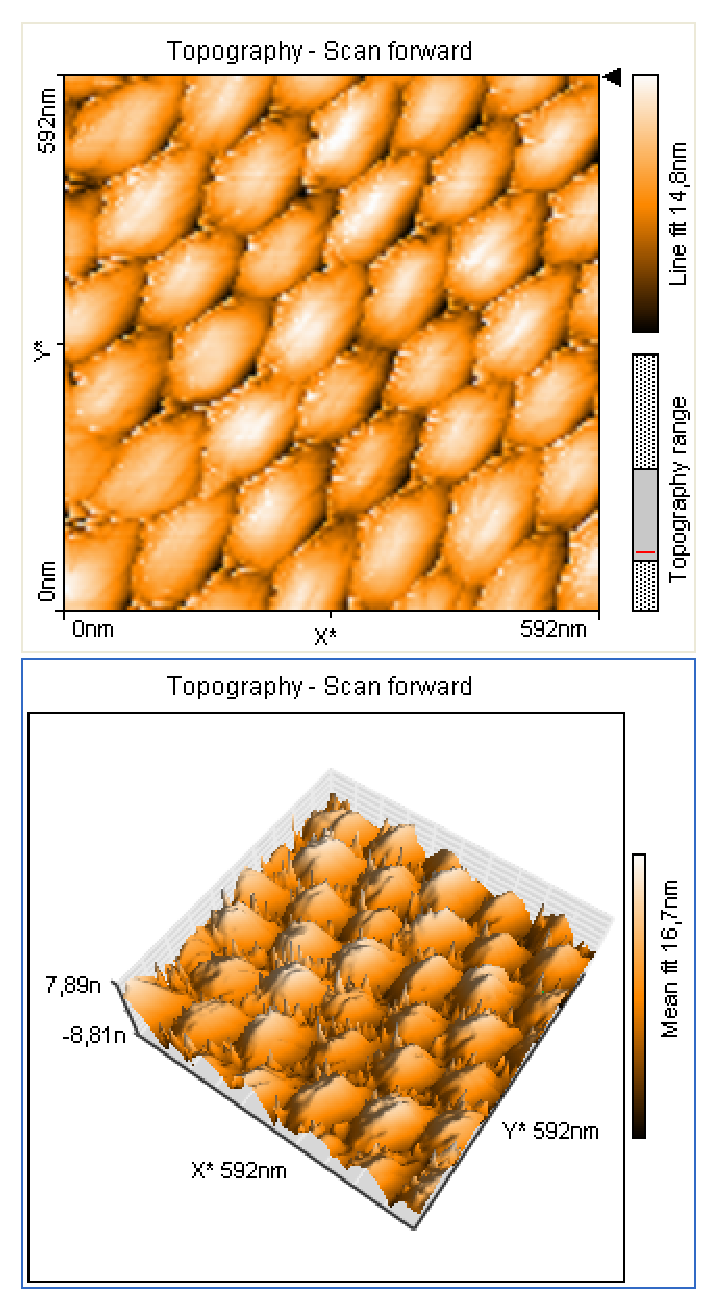
\includegraphics[width=0.9\linewidth]{../plot/data/goldgitter/goldgitter3.eps}
\end{minipage}
\begin{minipage}{0.2\linewidth}
\centering
\end{minipage}
\begin{minipage}{0.4\linewidth}
\centering
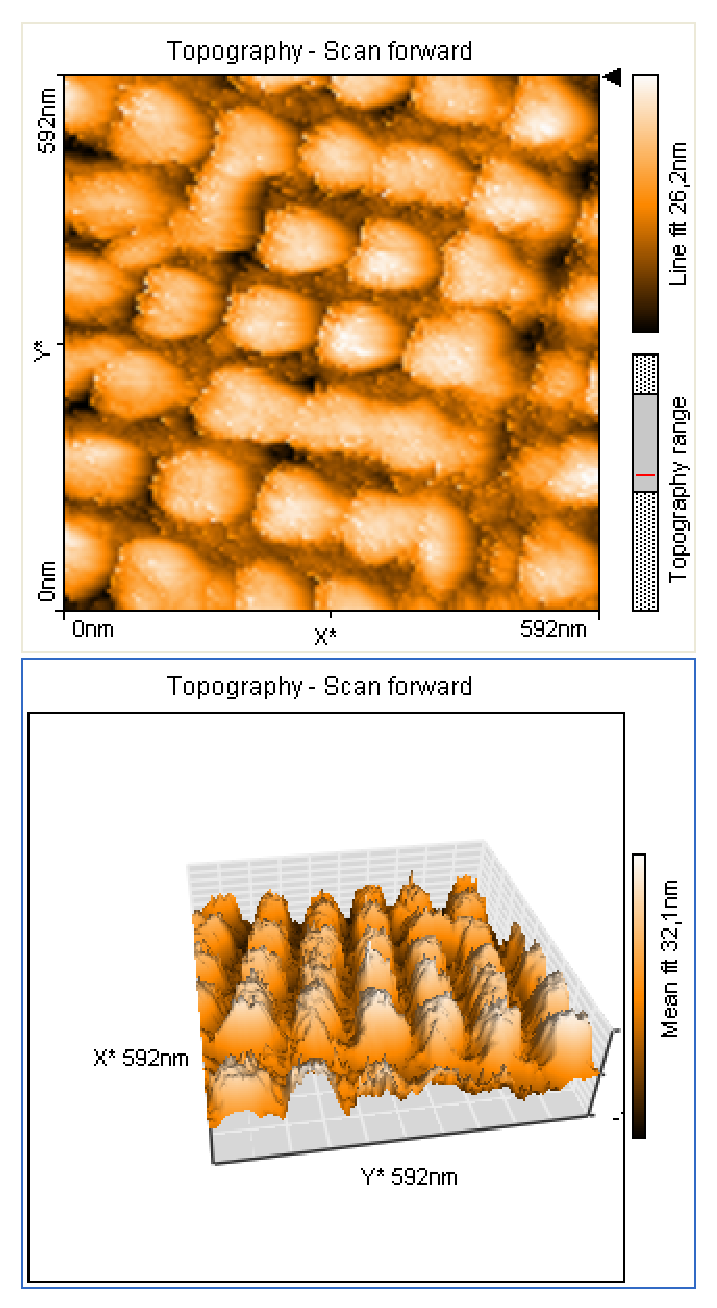
\includegraphics[width=0.9\linewidth]{../plot/data/goldgitter/goldgitter4.eps}
\end{minipage}
\end{figure}

\begin{figure}[H]  
\begin{minipage}{0.4\linewidth}
\centering
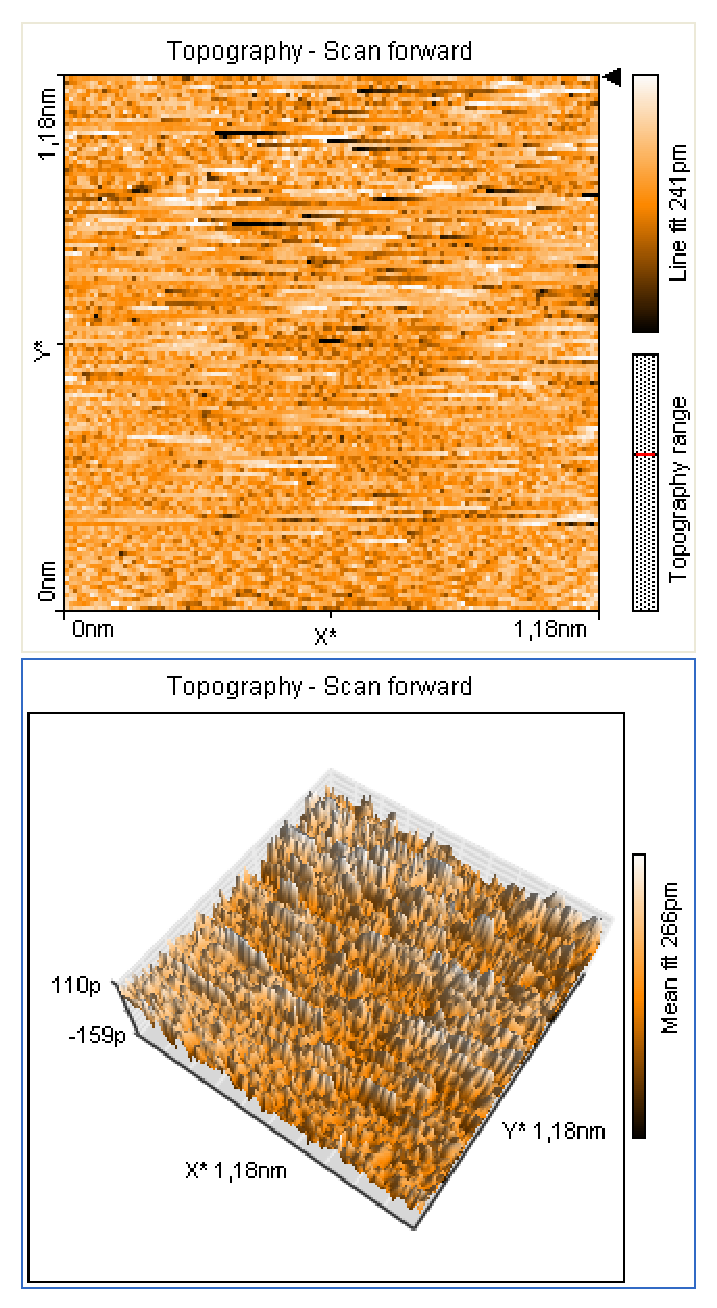
\includegraphics[width=0.9\linewidth]{../plot/data/goldgitter/goldgitter5.eps}
\end{minipage}
\begin{minipage}{0.2\linewidth}
\centering
\end{minipage}
\begin{minipage}{0.4\linewidth}
\centering
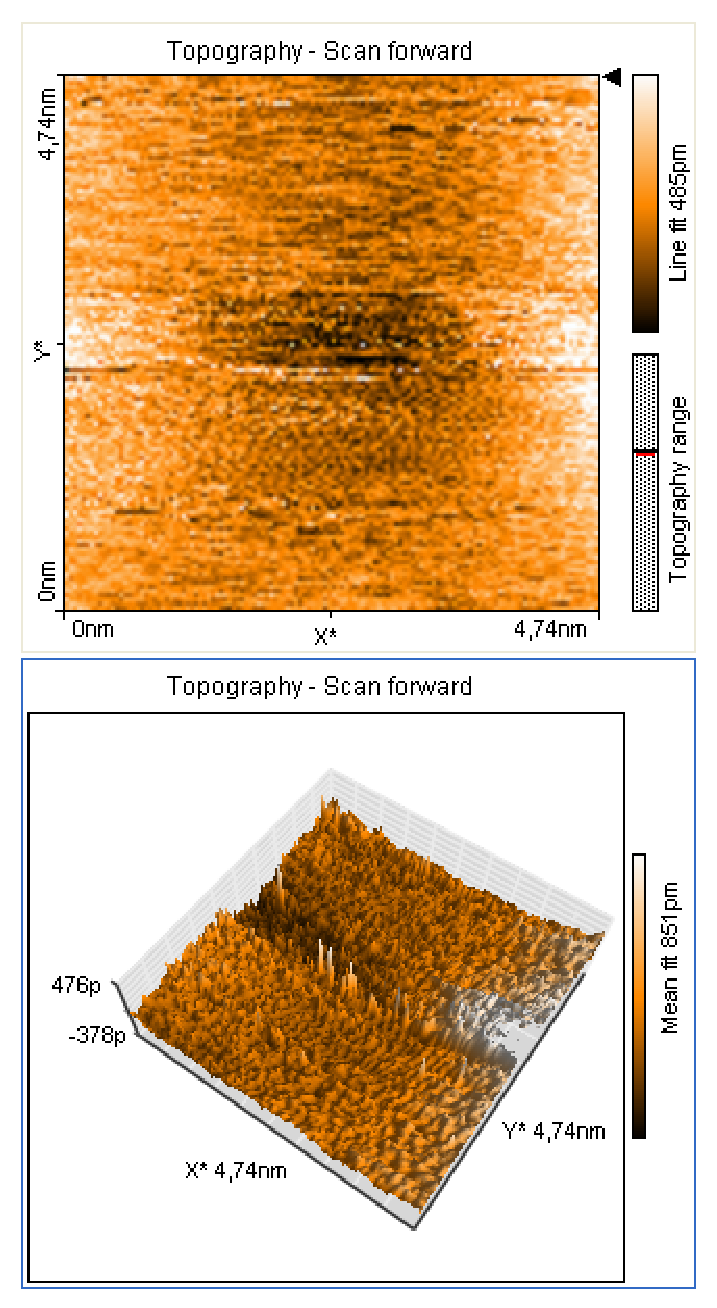
\includegraphics[width=0.9\linewidth]{../plot/data/goldgitter/goldgitter6.eps}
\end{minipage}
\end{figure}

\begin{figure}[H]  
\begin{minipage}{0.4\linewidth}
\centering
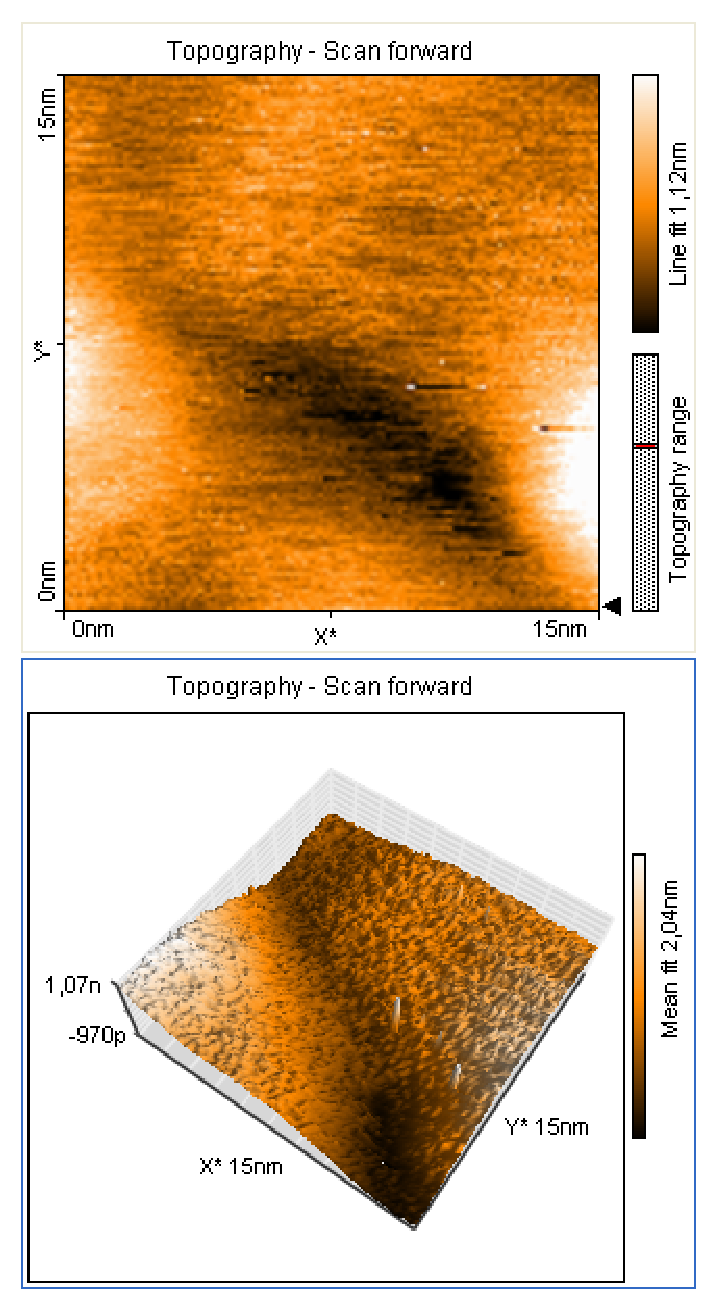
\includegraphics[width=0.9\linewidth]{../plot/data/goldgitter/goldgitter7.eps}
\end{minipage}
\begin{minipage}{0.2\linewidth}
\centering
\end{minipage}
\begin{minipage}{0.4\linewidth}
\centering
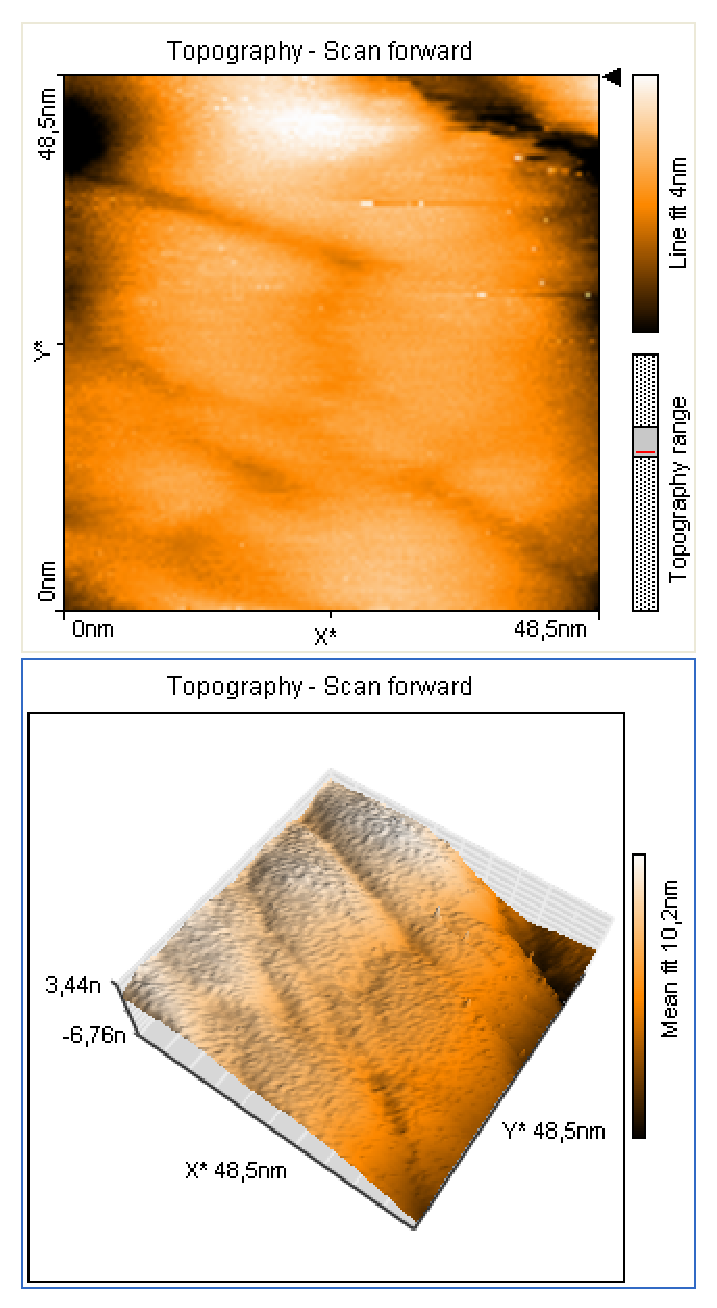
\includegraphics[width=0.9\linewidth]{../plot/data/goldgitter/goldgitter8.eps}
\end{minipage}
\end{figure}

Bei den vier besten Bildern haben wir mit der vorhandenen Software die Gitterabstände ausgemessen. In jedem Bild haben wir mindestens 3 Werte pro Richtung gemessen und aus diesen einen Mittelwert gebildet. Somit erhielten wir 8 Werte für die Gitterabstände beim Goldgitter, der Mittelwert aus diesen beträgt:
\begin{align*}
 d_{gold} = 102 \pm 11 nm
\end{align*}

\subsection{Graphit}

\begin{figure}[H]  
\begin{minipage}{0.4\linewidth}
\centering
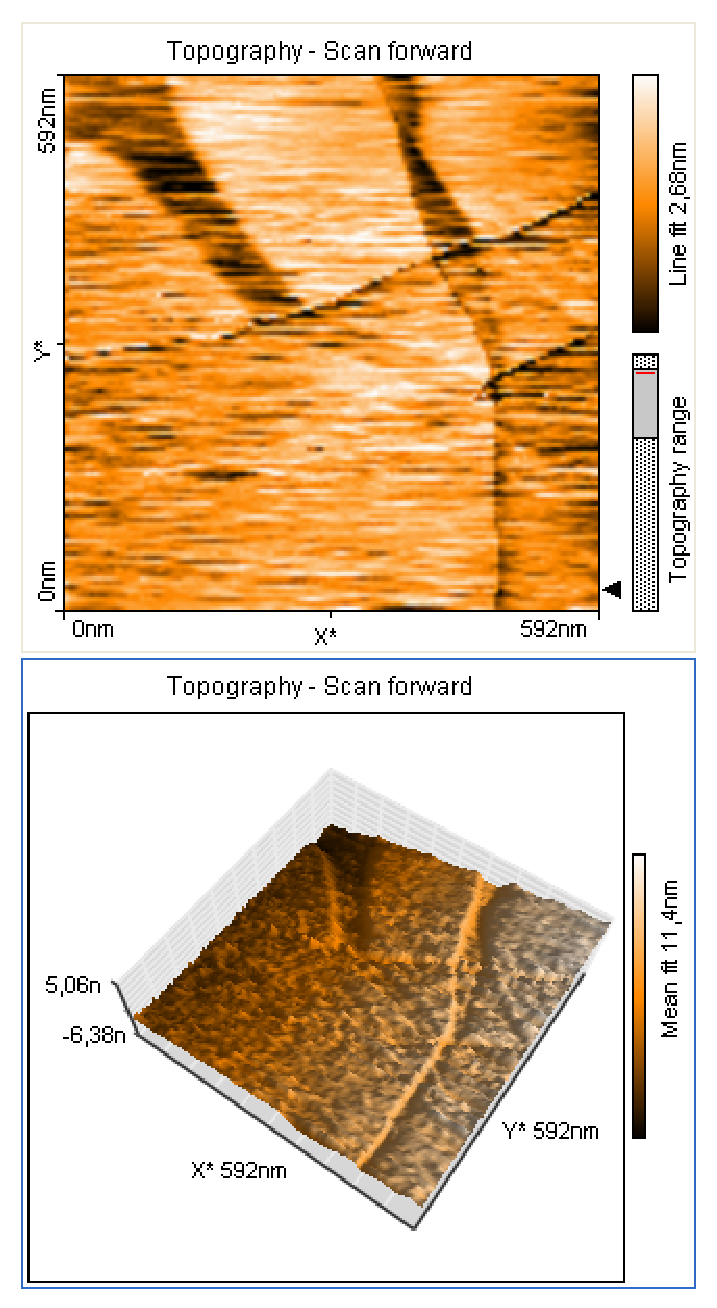
\includegraphics[width=0.9\linewidth]{../plot/data/graphit/graphit.eps}
\end{minipage}
\begin{minipage}{0.2\linewidth}
\centering
\end{minipage}
\begin{minipage}{0.4\linewidth}
\centering
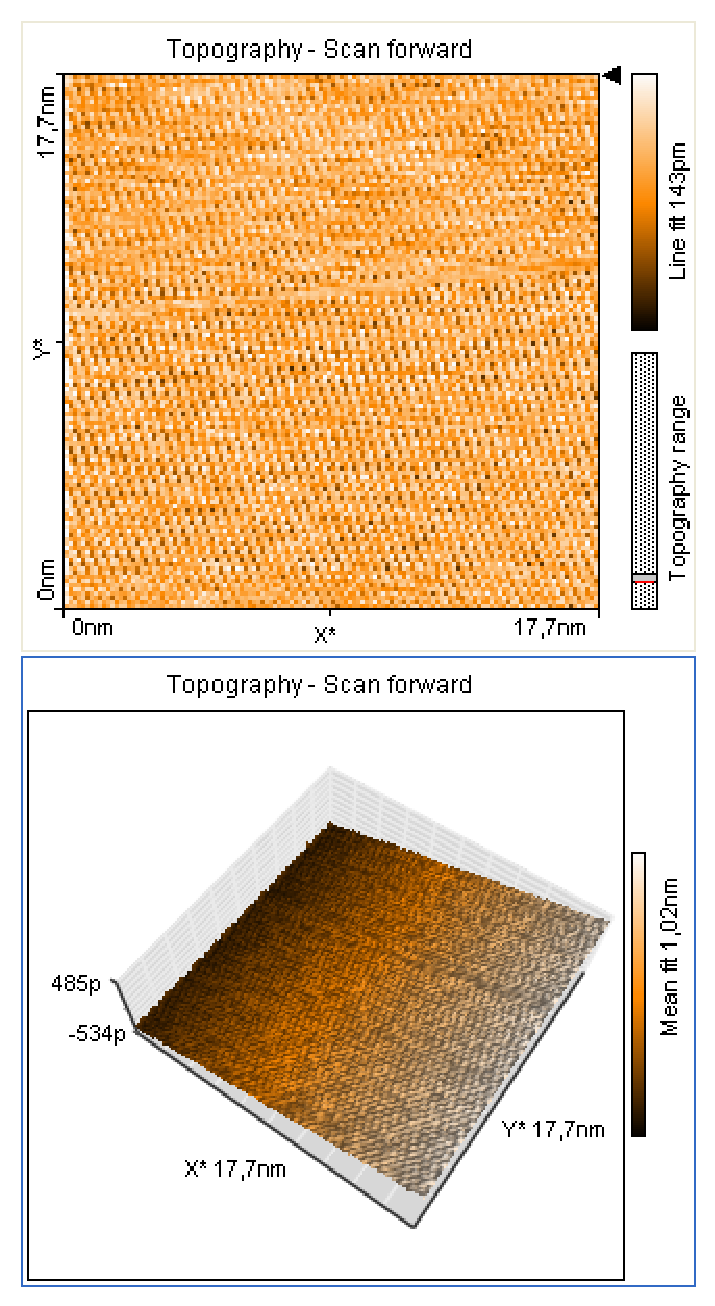
\includegraphics[width=0.9\linewidth]{../plot/data/graphit/graphit2.eps}
\end{minipage}
\end{figure}

\begin{figure}[H]  
\begin{minipage}{0.4\linewidth}
\centering
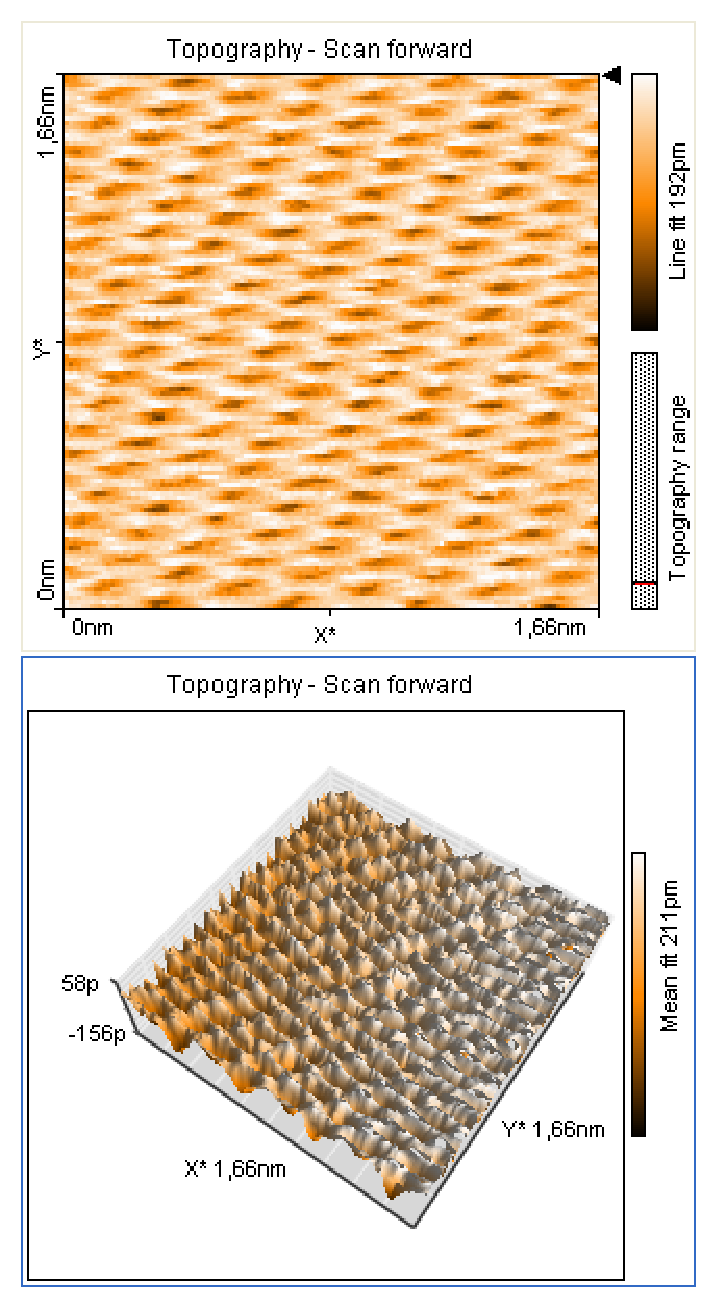
\includegraphics[width=0.9\linewidth]{../plot/data/graphit/graphit3.eps}
\end{minipage}
\begin{minipage}{0.2\linewidth}
\centering
\end{minipage}
\begin{minipage}{0.4\linewidth}
\centering
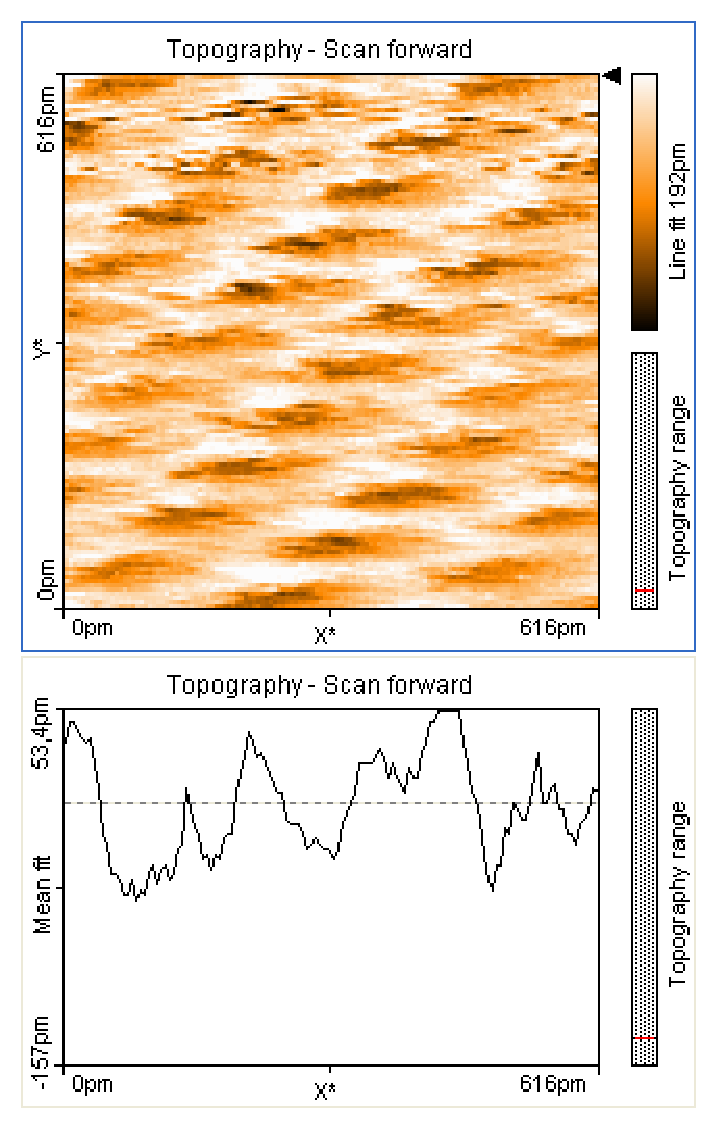
\includegraphics[width=0.9\linewidth]{../plot/data/graphit/graphit4.eps}
\end{minipage}
\end{figure}

\begin{figure}[H]  
\begin{minipage}{0.4\linewidth}
\centering
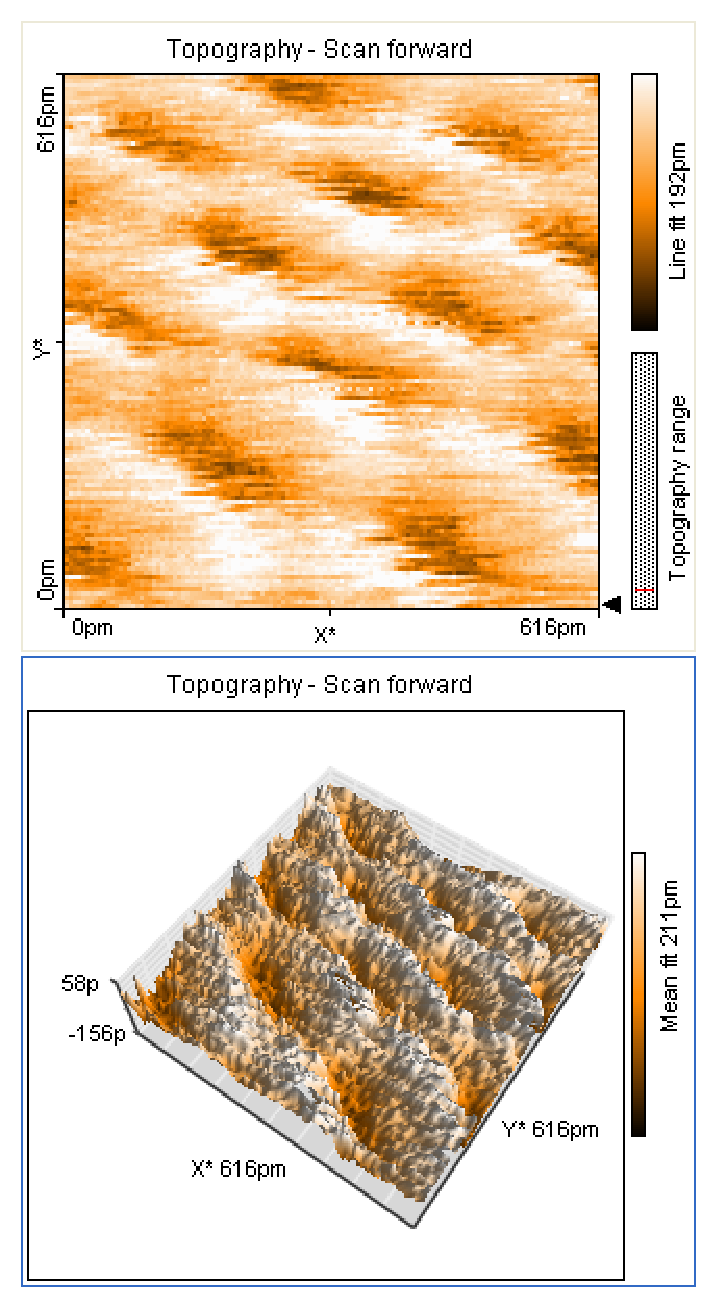
\includegraphics[width=0.9\linewidth]{../plot/data/graphit/graphit4-2.eps}
\end{minipage}
\begin{minipage}{0.2\linewidth}
\centering
\end{minipage}
\begin{minipage}{0.4\linewidth}
\centering
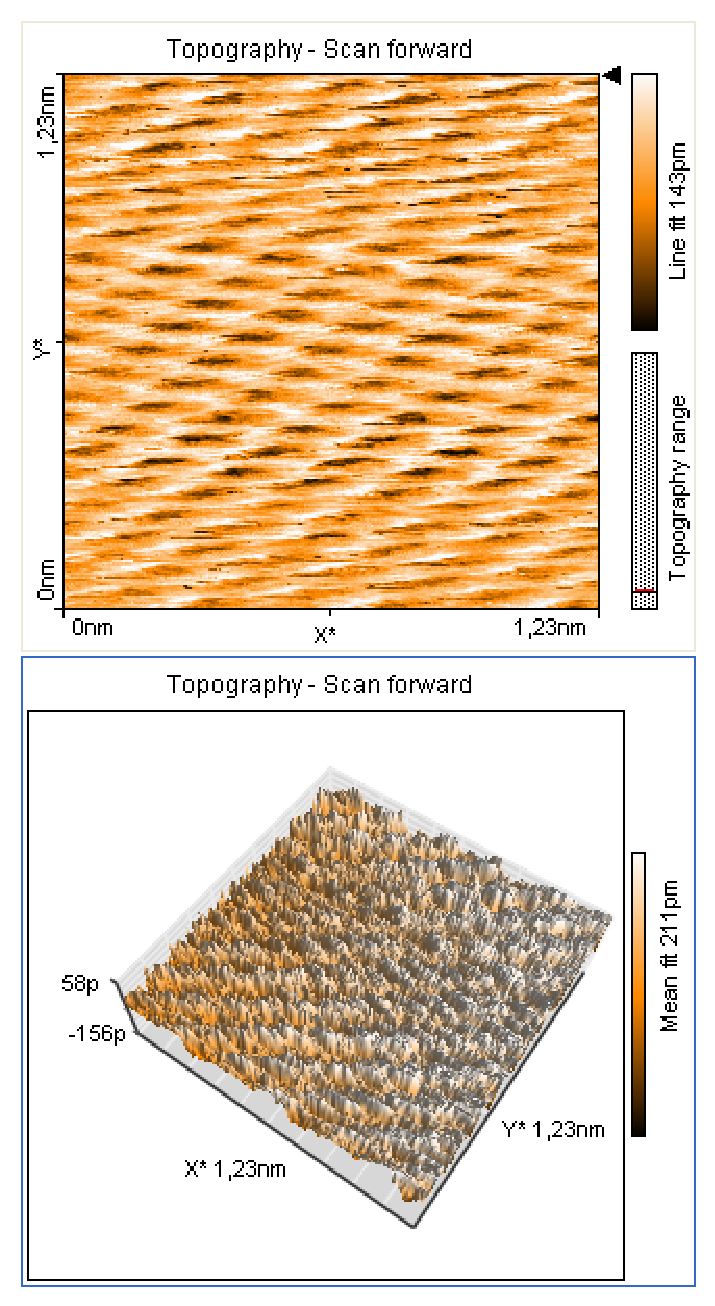
\includegraphics[width=0.9\linewidth]{../plot/data/graphit/graphit5.eps}
\end{minipage}
\end{figure}

Wie beim Goldgitter haben wir auch hier mit der Software die Abstände vermessen. Bei Graphit unterscheiden sich jedoch die Abstände in den verschiedenen Richtungen:
\begin{align*}
 d_1 &= 130 \pm 15 pm \\
 d_2 &= 67 \pm 6 pm \\
 d_3 &= 66 \pm 23 pm
\end{align*}

\subsection{Molybdändisulfid}

\begin{figure}[H]  
\begin{minipage}{0.4\linewidth}
\centering
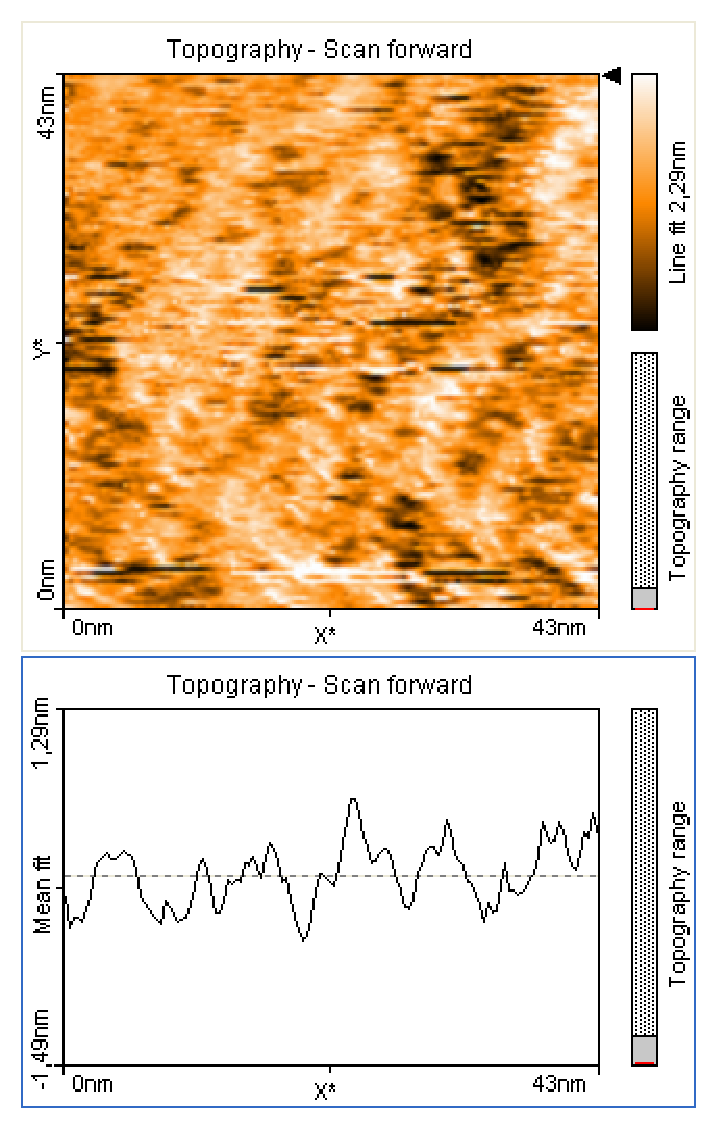
\includegraphics[width=0.9\linewidth]{../plot/data/mos2/mos2.eps}
\end{minipage}
\begin{minipage}{0.2\linewidth}
\centering
\end{minipage}
\begin{minipage}{0.4\linewidth}
\centering
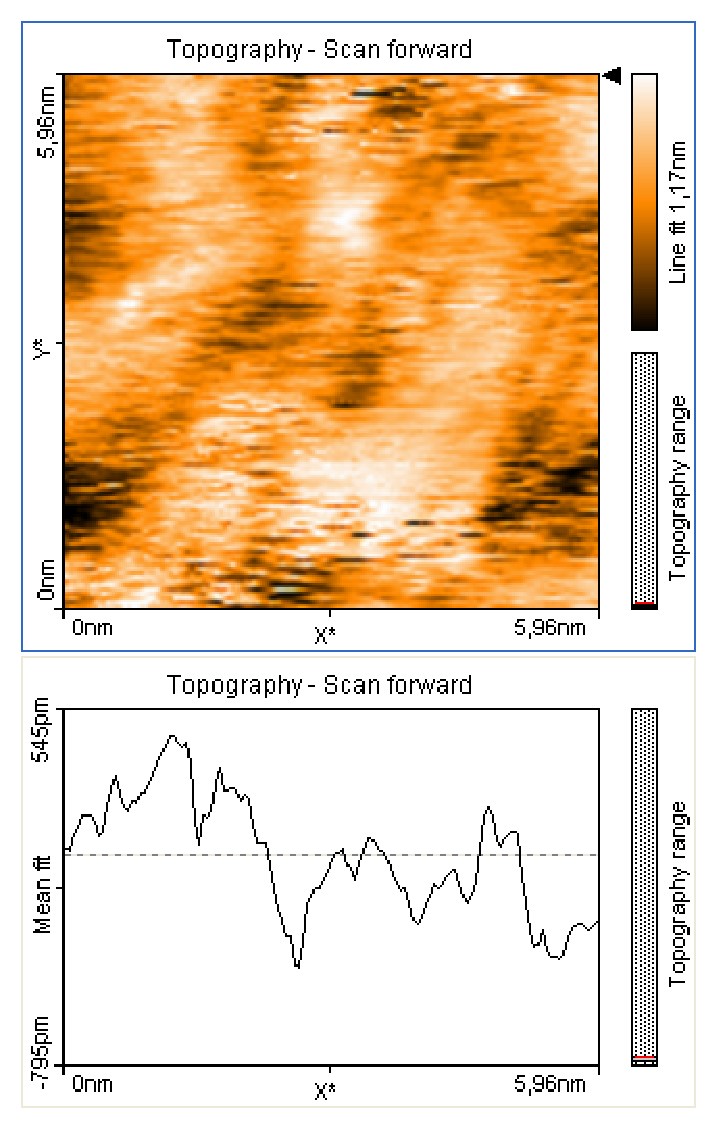
\includegraphics[width=0.9\linewidth]{../plot/data/mos2/mos21.eps}
\end{minipage}
\end{figure}

\begin{figure}[H]  
\begin{minipage}{0.4\linewidth}
\centering
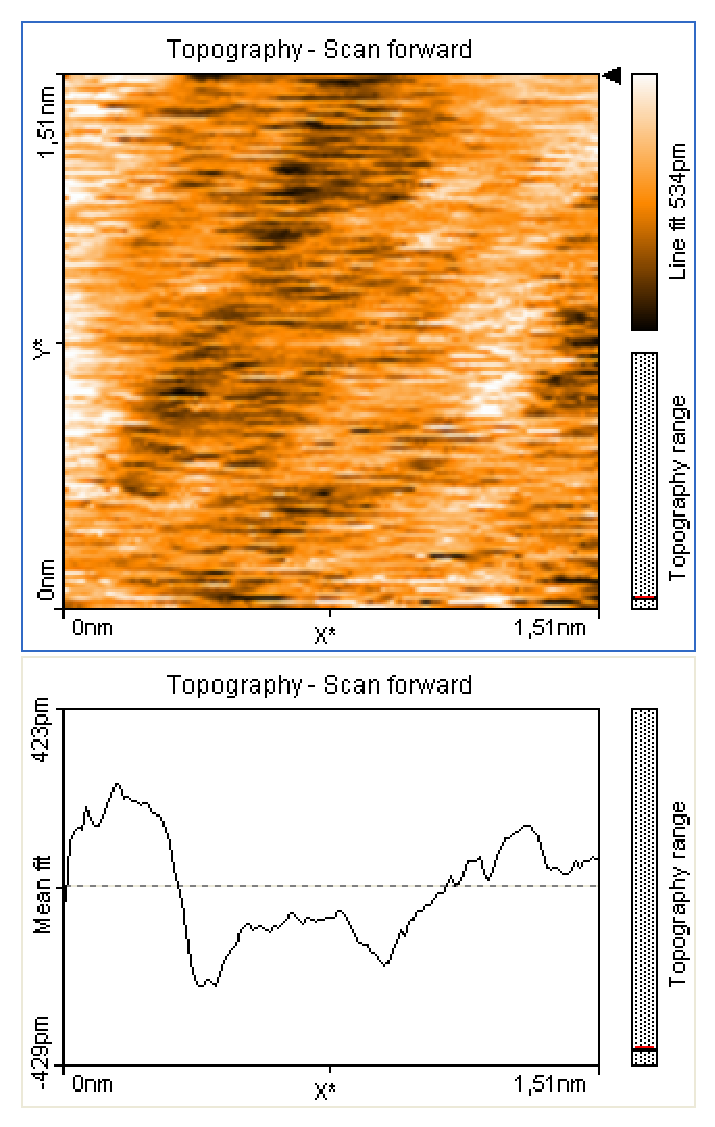
\includegraphics[width=0.9\linewidth]{../plot/data/mos2/mos22.eps}
\end{minipage}
\begin{minipage}{0.2\linewidth}
\centering
\end{minipage}
\begin{minipage}{0.4\linewidth}
\centering
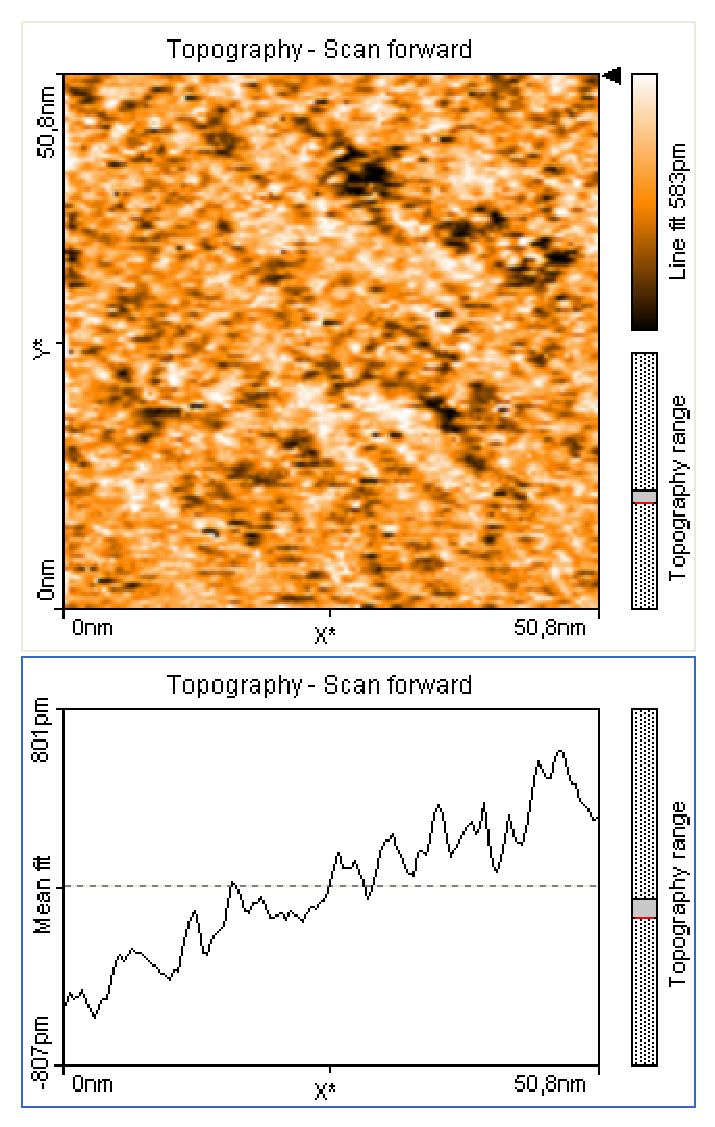
\includegraphics[width=0.9\linewidth]{../plot/data/mos2/mos23.eps}
\end{minipage}
\end{figure}

\begin{figure}[H]  
\begin{minipage}{0.4\linewidth}
\centering
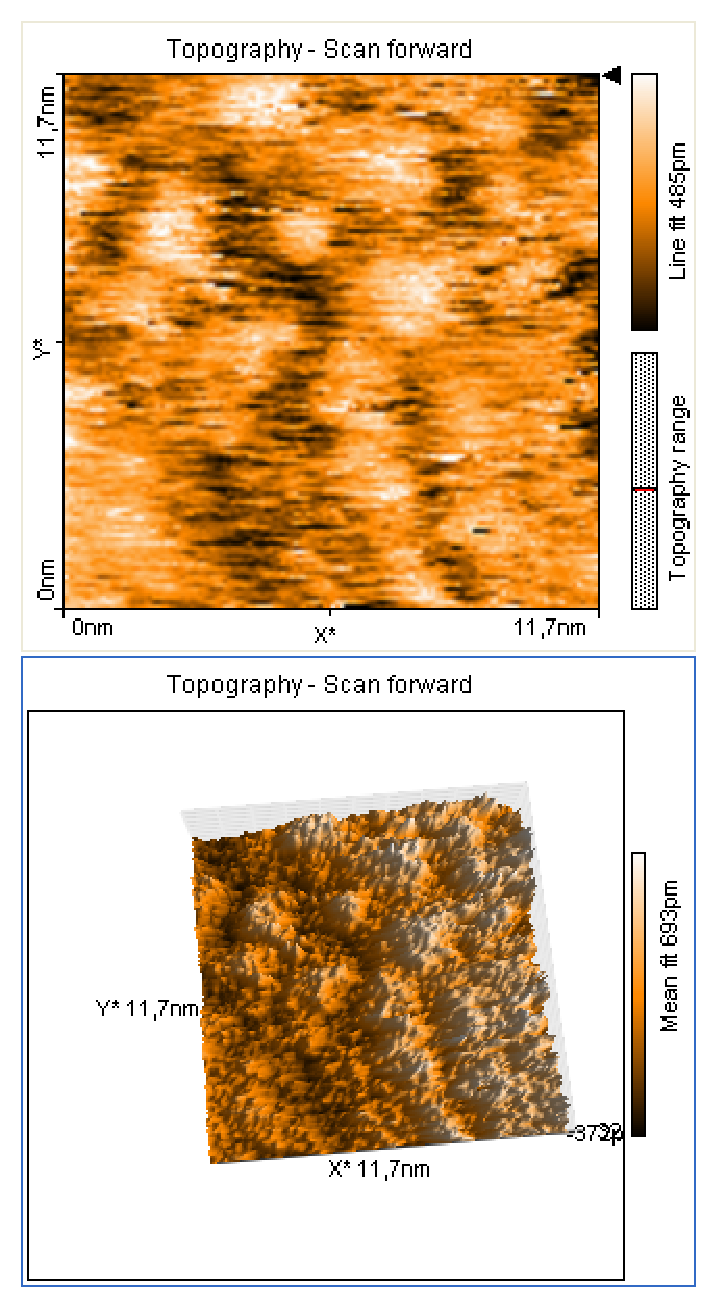
\includegraphics[width=0.9\linewidth]{../plot/data/mos2/mos24.eps}
\end{minipage}
\begin{minipage}{0.2\linewidth}
\centering
\end{minipage}
\begin{minipage}{0.4\linewidth}
\centering
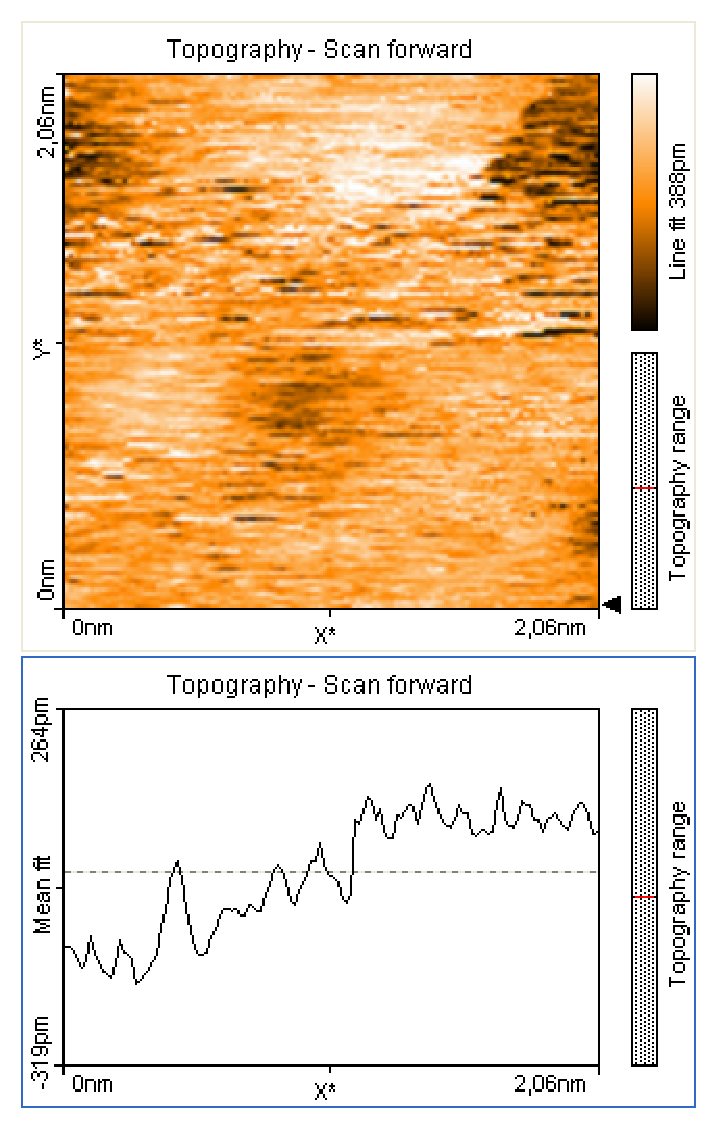
\includegraphics[width=0.9\linewidth]{../plot/data/mos2/mos25.eps}
\end{minipage}
\end{figure}

\begin{figure}[H]  
\begin{minipage}{0.4\linewidth}
\centering
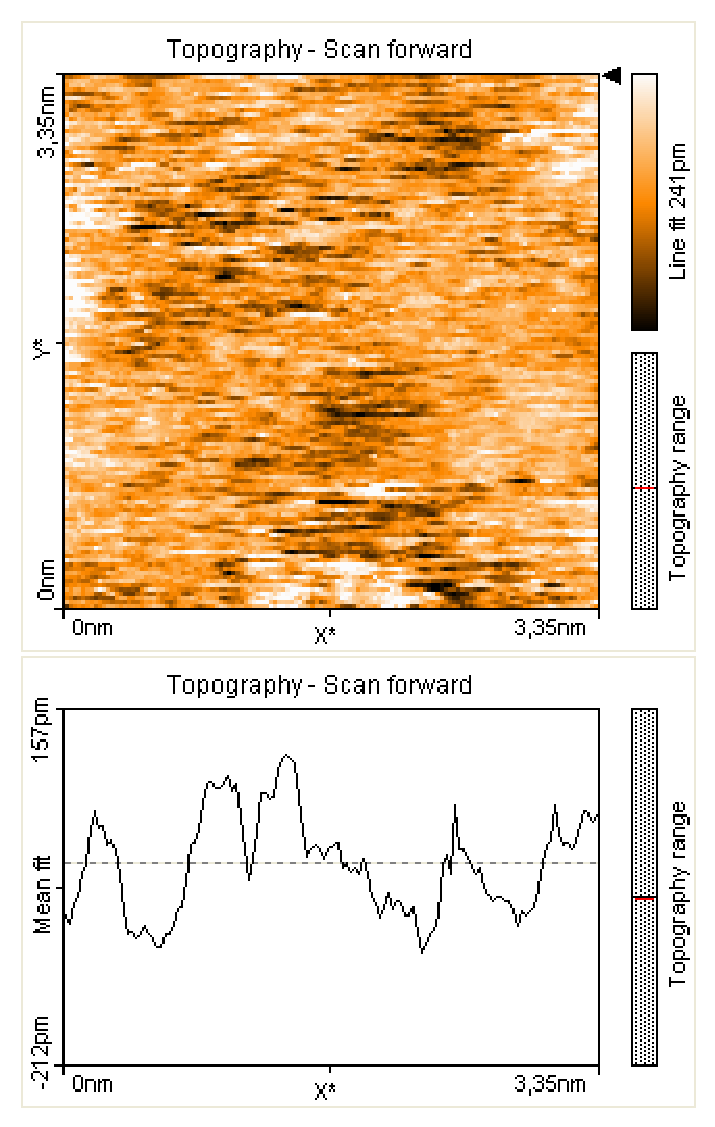
\includegraphics[width=0.9\linewidth]{../plot/data/mos2/mos26.eps}
\end{minipage}
\begin{minipage}{0.2\linewidth}
\centering
\end{minipage}
\begin{minipage}{0.4\linewidth}
\centering
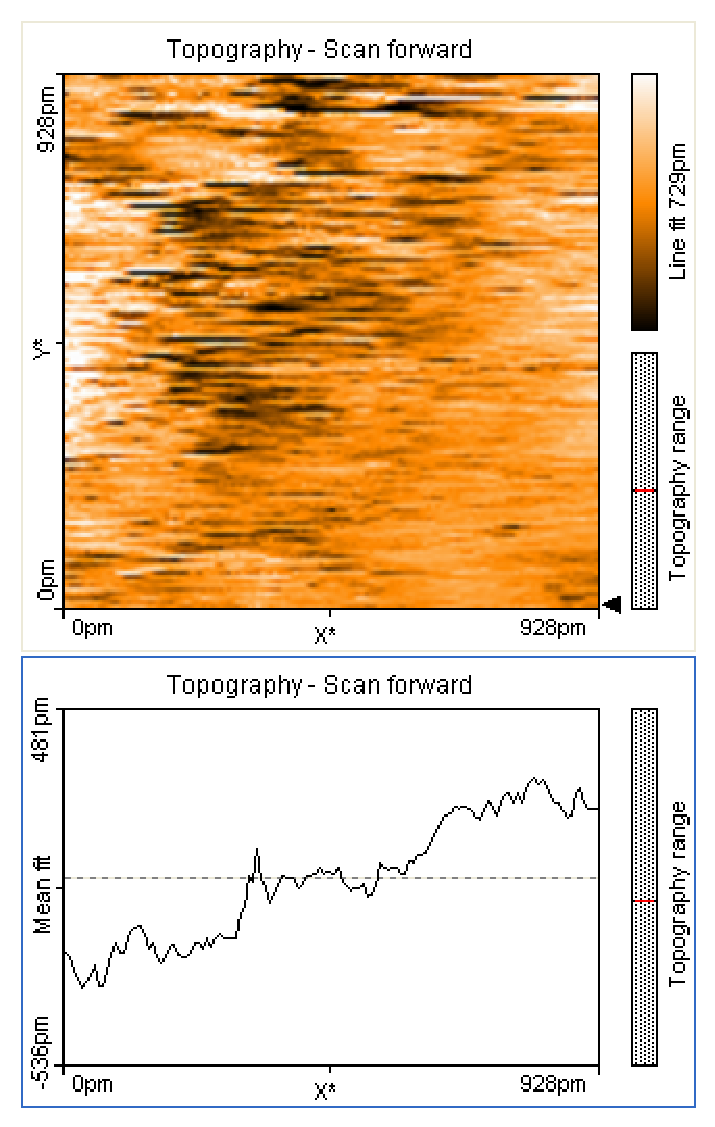
\includegraphics[width=0.9\linewidth]{../plot/data/mos2/mos27.eps}
\end{minipage}
\end{figure}

\begin{figure}[H]  
\begin{minipage}{0.4\linewidth}
\centering
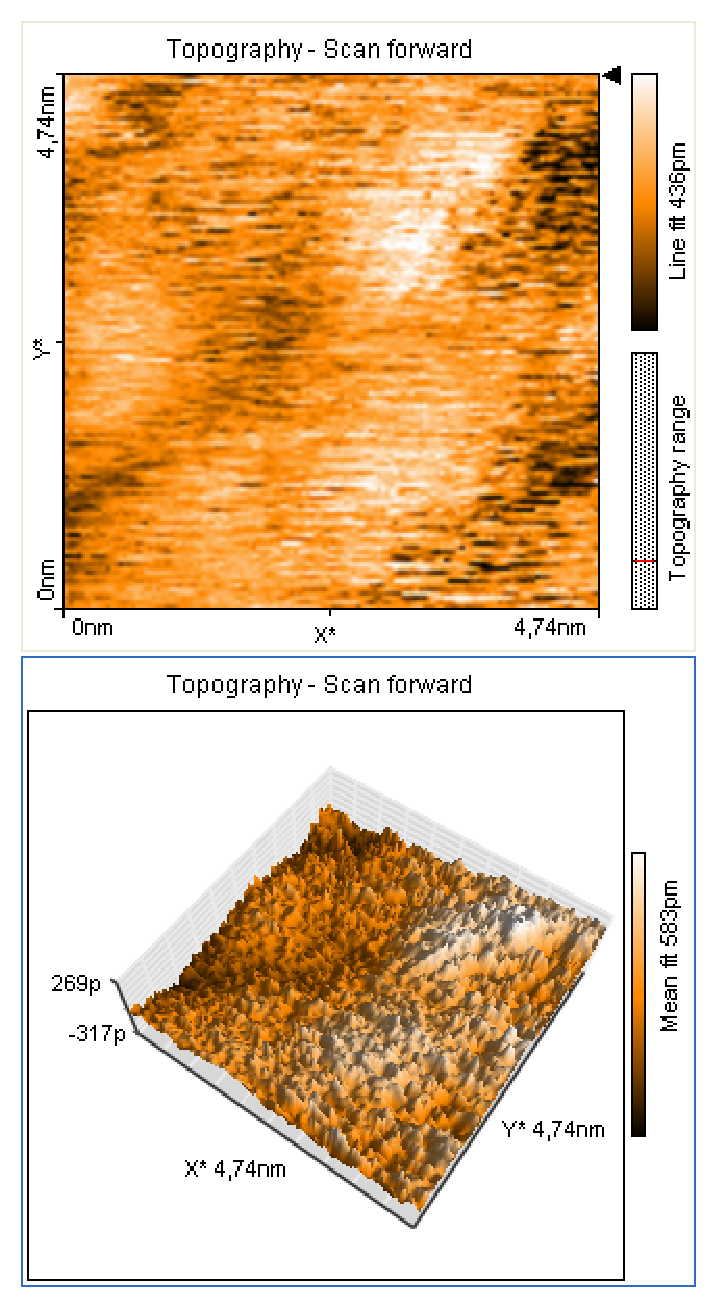
\includegraphics[width=0.9\linewidth]{../plot/data/mos2/mos28.eps}
\end{minipage}
\begin{minipage}{0.2\linewidth}
\centering
\end{minipage}
\begin{minipage}{0.4\linewidth}
\centering
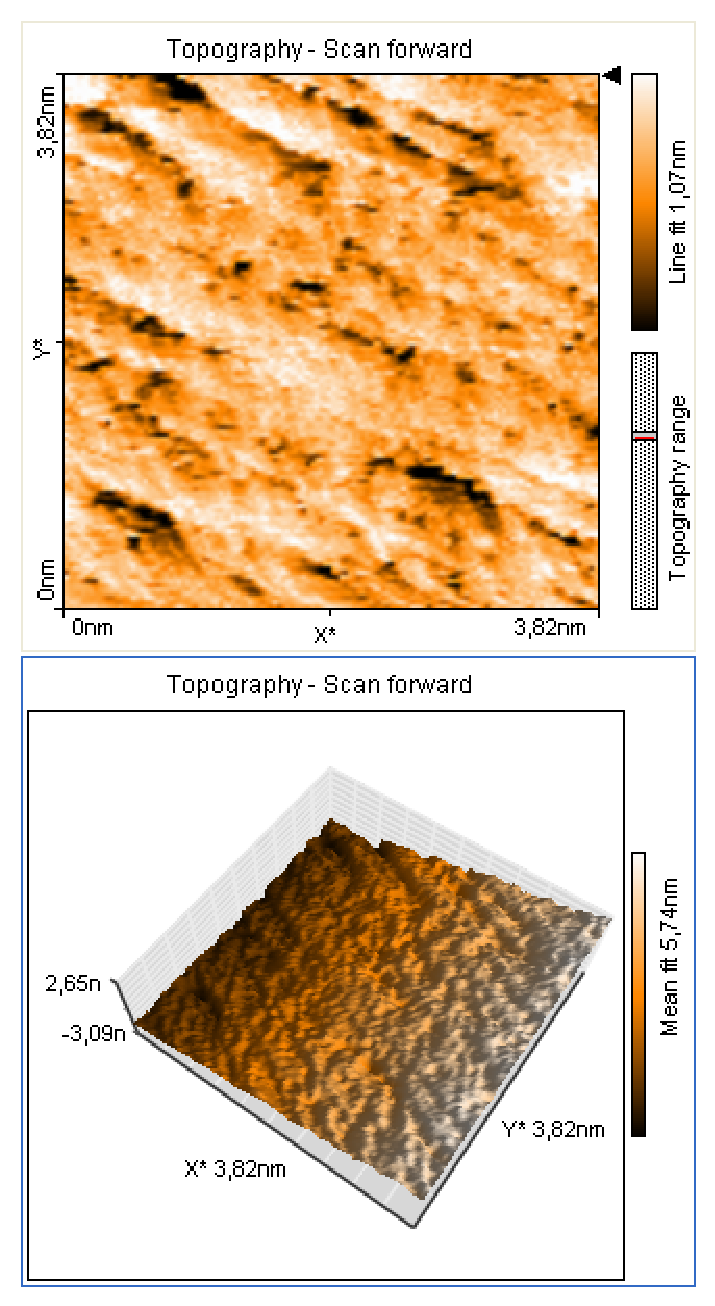
\includegraphics[width=0.9\linewidth]{../plot/data/mos2/mos29.eps}
\end{minipage}
\end{figure}

Wie man an den Bildern erkennen kann stellte sich das Ausmessen der Abstände bei $MoS_2$ als schwierig heraus. Für die Orientierung die wir einigermaßen erkennen konnten ergibt sich im Mittel:
\begin{align*}
 d_{MoS_2} = 914 \pm 26 pm
\end{align*}


\section{Zusammenfassung}
Der Umgang mit dem Rastertunnelmikroskop erscheint auf den ersten Blick einfach, jedoch stellt man bald fest, das gute Bilder nur mit ausreichender Geduld und einiger Übung zu bekommen sind. Es frustriert zu sehen wie das Gerät die gerade hergestellte Spitze die so vielversprechend unter dem Vergrößerungsglas aussah gegen die Probe fährt. Oder man verzweifelt beim Warten dass der Annäherungsvorgang endlich abgeschlossen ist, wenn man dann von Hand doch noch ein bisschen näher an die Spitze fahren will landet man meistens doch schon darin. Hat man es schließlich mal geschafft und der richtige Abstand ist gefunden so muss man oft feststellen das die Stelle der Probe an der man die Spitze hat nicht plan genug ist um das zu sehen was man sucht, also beginnt die ganze Prozedur von vorne. Einige Spitzen und viele Nerven später hat man dann endlich das erhoffte Bild. Leider hat man wohl die das Glück, dass die Spitze genau senkrecht auf die Kristallstruktur steht, wenn man jedoch versucht die Winkeleinstellungen zu ändern um dies auszugleichen so stellt man bald fest, dass es nur noch schlimmer wird und die Spitze dann alsbald wieder in die Probe fährt. Schlussendlich verbringt man anderthalb Tage damit auf das Glück zu warten einmal ein gutes Bild zu machen. Nach dieser Zeit und ca. $15cm$ Platindraht haben wir zwei duzend Bilder die Qualitativ nicht an das heranreichen was man von anderen Quellen her kennt. Ein relativ ernüchterndes Ergebnis.

Es war trotzdem interessant einmal mit einem Rastertunnelmikroskop zu arbeiten und man wird die Arbeit die hinter einer guten Aufnahme steckt sicher nicht mehr unterschätzen.\\

Ein exaktes Ausmessen der Abstände der Gitterpunkte bzw. Atome stellte sich als schwierig heraus, es ist mehr eine ``pi-mal-Daumen'' Angelegenheit. Hier muss man eben viele Messungen machen um die Fehler akzeptabel zu halten.

Die angegeben Gitterkonstante des Goldgitters konnten wir, wie auch andere, nicht verifizieren. Das Gitter scheint den Bildern nach aber auch nicht mehr das zu sein welches in der Staatsexamensarbeit abgebildet ist.\\

Die von uns vermessenen Werte:
\begin{align*}
 d_{gold} &= 102 \pm 11 nm \\
 &\textnormal{Graphit:} \\
 d_1 &= 130 \pm 15 pm \\
 d_2 &= 67 \pm 6 pm \\
 d_3 &= 66 \pm 23 pm \\
 d_{MoS_2} &= 914 \pm 26 pm
\end{align*}


\end{document}
